\documentclass[11pt,fleqn]{book} % Default font size and left-justified equations
\usepackage{minted}
\usepackage{listings}
\usepackage{hyperref}
\usepackage[top=3cm,bottom=3cm,left=3.2cm,right=3.2cm,headsep=10pt,letterpaper]{geometry} % Page margins
\setlength{\headheight}{25.85pt} 

\usepackage{xcolor} % Required for specifying colors by name
\definecolor{ocre}{RGB}{52,177,201} % Define the orange color used for highlighting throughout the book

% Font Settings
\usepackage{avant}
\usepackage{mathptmx}
\usepackage{url}
\newcounter{mycounter}
\setcounter{mycounter}{1}
\newcounter{question}
\setcounter{question}{1}

\usepackage{microtype} % Slightly tweak font spacing for aesthetics
\usepackage[utf8]{inputenc} % Required for including letters with accents
\usepackage[T1]{fontenc} % Use 8-bit encoding that has 256 glyphs

\renewcommand{\lstlistingname}{Code}

% Bibliography
%\usepackage[style=alphabetic,sorting=nyt,sortcites=true,autopunct=true,autolang=hyphen,hyperref=true,abbreviate=false,backref=true,backend=biber]{biblatex}
%\addbibresource{bibliography.bib} % BibTeX bibliography file
%\defbibheading{bibempty}{}

%----------------------------------------------------------------------------------------
%	VARIOUS REQUIRED PACKAGES
%----------------------------------------------------------------------------------------

\usepackage{titlesec} % Allows customization of titles

\usepackage{graphicx} % Required for including pictures
\graphicspath{{Pictures/}} % Specifies the directory where pictures are stored

\usepackage{lipsum} % Inserts dummy text

\usepackage{tikz} % Required for drawing custom shapes

\usepackage[english]{babel} % English language/hyphenation

\usepackage{enumitem} % Customize lists
\setlist{nolistsep} % Reduce spacing between bullet points and numbered lists

\usepackage{booktabs} % Required for nicer horizontal rules in tables

\usepackage{eso-pic} % Required for specifying an image background in the title page

%----------------------------------------------------------------------------------------
%	MAIN TABLE OF CONTENTS
%----------------------------------------------------------------------------------------

\usepackage{titletoc} % Required for manipulating the table of contents

\contentsmargin{0cm} % Removes the default margin
% Chapter text styling
\titlecontents{chapter}[1.25cm] % Indentation
{\addvspace{15pt}\large\sffamily\bfseries} % Spacing and font options for chapters
{\color{ocre!60}\contentslabel[\Large\thecontentslabel]{1.25cm}\color{ocre}} % Chapter number
{}  
{\color{ocre!60}\normalsize\sffamily\bfseries\;\titlerule*[.5pc]{.}\;\thecontentspage} % Page number
% Section text styling
\titlecontents{section}[1.25cm] % Indentation
{\addvspace{5pt}\sffamily\bfseries} % Spacing and font options for sections
{\contentslabel[\thecontentslabel]{1.25cm}} % Section number
{}
{\sffamily\hfill\color{black}\thecontentspage} % Page number
[]
% Subsection text styling
\titlecontents{subsection}[1.25cm] % Indentation
{\addvspace{1pt}\sffamily\small} % Spacing and font options for subsections
{\contentslabel[\thecontentslabel]{1.25cm}} % Subsection number
{}
{\sffamily\;\titlerule*[.5pc]{.}\;\thecontentspage} % Page number
[] 

%----------------------------------------------------------------------------------------
%	MINI TABLE OF CONTENTS IN CHAPTER HEADS
%----------------------------------------------------------------------------------------

% Section text styling
\titlecontents{lsection}[0em] % Indendating
{\footnotesize\sffamily} % Font settings
{}
{}
{}

% Subsection text styling
\titlecontents{lsubsection}[.5em] % Indentation
{\normalfont\footnotesize\sffamily} % Font settings
{}
{}
{}
 
%----------------------------------------------------------------------------------------
%	PAGE HEADERS
%----------------------------------------------------------------------------------------

\usepackage{fancyhdr} % Required for header and footer configuration

\pagestyle{fancy}
\renewcommand{\chaptermark}[1]{\markboth{\sffamily\normalsize\bfseries\chaptername\ \thechapter.\ #1}{}} % Chapter text font settings
\renewcommand{\sectionmark}[1]{\markright{\sffamily\normalsize\thesection\hspace{5pt}#1}{}} % Section text font settings
\fancyhf{} \fancyhead[LE,RO]{\sffamily\normalsize\thepage} % Font setting for the page number in the header
\fancyhead[LO]{\rightmark} % Print the nearest section name on the left side of odd pages
\fancyhead[RE]{\leftmark} % Print the current chapter name on the right side of even pages
\renewcommand{\headrulewidth}{0.5pt} % Width of the rule under the header
\addtolength{\headheight}{2.5pt} % Increase the spacing around the header slightly
\renewcommand{\footrulewidth}{0pt} % Removes the rule in the footer
\fancypagestyle{plain}{\fancyhead{}\renewcommand{\headrulewidth}{0pt}} % Style for when a plain pagestyle is specified

% Removes the header from odd empty pages at the end of chapters
\makeatletter
\renewcommand{\cleardoublepage}{
\clearpage\ifodd\c@page\else
\hbox{}
\vspace*{\fill}
\thispagestyle{empty}
\newpage
\fi}

%----------------------------------------------------------------------------------------
%	THEOREM STYLES
%----------------------------------------------------------------------------------------

\usepackage{amsmath,amsfonts,amssymb,amsthm} % For math equations, theorems, symbols, etc

\newcommand{\intoo}[2]{\mathopen{]}#1\,;#2\mathclose{[}}
\newcommand{\ud}{\mathop{\mathrm{{}d}}\mathopen{}}
\newcommand{\intff}[2]{\mathopen{[}#1\,;#2\mathclose{]}}
\newtheorem{notation}{Notation}[chapter]

%%%%%%%%%%%%%%%%%%%%%%%%%%%%%%%%%%%%%%%%%%%%%%%%%%%%%%%%%%%%%%%%%%%%%%%%%%%
%%%%%%%%%%%%%%%%%%%% dedicated to boxed/framed environements %%%%%%%%%%%%%%
%%%%%%%%%%%%%%%%%%%%%%%%%%%%%%%%%%%%%%%%%%%%%%%%%%%%%%%%%%%%%%%%%%%%%%%%%%%
\newtheoremstyle{ocrenumbox}% % Theorem style name
{0pt}% Space above
{0pt}% Space below
{\normalfont}% % Body font
{}% Indent amount
{\small\bf\sffamily\color{ocre}}% % Theorem head font
{\;}% Punctuation after theorem head
{0.25em}% Space after theorem head
{\small\sffamily\color{ocre}\thmname{#1}\nobreakspace\thmnumber{\@ifnotempty{#1}{}\@upn{#2}}% Theorem text (e.g. Theorem 2.1)
\thmnote{\nobreakspace\the\thm@notefont\sffamily\bfseries\color{black}---\nobreakspace#3.}} % Optional theorem note
\renewcommand{\qedsymbol}{$\blacksquare$}% Optional qed square

\newtheoremstyle{blacknumex}% Theorem style name
{5pt}% Space above
{5pt}% Space below
{\normalfont}% Body font
{} % Indent amount
{\small\bf\sffamily}% Theorem head font
{\;}% Punctuation after theorem head
{0.25em}% Space after theorem head
{\small\sffamily{\tiny\ensuremath{\blacksquare}}\nobreakspace\thmname{#1}\nobreakspace\thmnumber{\@ifnotempty{#1}{}\@upn{#2}}% Theorem text (e.g. Theorem 2.1)
\thmnote{\nobreakspace\the\thm@notefont\sffamily\bfseries---\nobreakspace#3.}}% Optional theorem note

\newtheoremstyle{blacknumbox} % Theorem style name
{0pt}% Space above
{0pt}% Space below
{\normalfont}% Body font
{}% Indent amount
{\small\bf\sffamily}% Theorem head font
{\;}% Punctuation after theorem head
{0.25em}% Space after theorem head
{\small\sffamily\thmname{#1}\nobreakspace\thmnumber{\@ifnotempty{#1}{}\@upn{#2}}% Theorem text (e.g. Theorem 2.1)
\thmnote{\nobreakspace\the\thm@notefont\sffamily\bfseries---\nobreakspace#3.}}% Optional theorem note

%%%%%%%%%%%%%%%%%%%%%%%%%%%%%%%%%%%%%%%%%%%%%%%%%%%%%%%%%%%%%%%%%%%%%%%%%%%
%%%%%%%%%%%%% dedicated to non-boxed/non-framed environements %%%%%%%%%%%%%
%%%%%%%%%%%%%%%%%%%%%%%%%%%%%%%%%%%%%%%%%%%%%%%%%%%%%%%%%%%%%%%%%%%%%%%%%%%
\newtheoremstyle{ocrenum}% % Theorem style name
{5pt}% Space above
{5pt}% Space below
{\normalfont}% % Body font
{}% Indent amount
{\small\bf\sffamily\color{ocre}}% % Theorem head font
{\;}% Punctuation after theorem head
{0.25em}% Space after theorem head
{\small\sffamily\color{ocre}\thmname{#1}\nobreakspace\thmnumber{\@ifnotempty{#1}{}\@upn{#2}}% Theorem text (e.g. Theorem 2.1)
\thmnote{\nobreakspace\the\thm@notefont\sffamily\bfseries\color{black}---\nobreakspace#3.}} % Optional theorem note
\renewcommand{\qedsymbol}{$\blacksquare$}% Optional qed square
\makeatother

% Defines the theorem text style for each type of theorem to one of the three styles above
\newcounter{dummy} 
\numberwithin{dummy}{section}
\theoremstyle{ocrenumbox}
\newtheorem{theoremeT}[dummy]{Theorem}
\newtheorem{problem}{Problem}[chapter]
\newtheorem{exerciseT}{Exercise}[chapter]
\theoremstyle{blacknumex}
\newtheorem{exampleT}{Example}[chapter]
\theoremstyle{blacknumbox}
\newtheorem{vocabulary}{Vocabulary}[chapter]
\newtheorem{definitionT}{Definition}[section]
\newtheorem{corollaryT}[dummy]{Corollary}
\theoremstyle{ocrenum}
\newtheorem{proposition}[dummy]{Proposition}

%----------------------------------------------------------------------------------------
%	DEFINITION OF COLORED BOXES
%----------------------------------------------------------------------------------------

\RequirePackage[framemethod=default]{mdframed} % Required for creating the theorem, definition, exercise and corollary boxes

% Theorem box
\newmdenv[skipabove=7pt,
skipbelow=7pt,
backgroundcolor=black!5,
linecolor=ocre,
innerleftmargin=5pt,
innerrightmargin=5pt,
innertopmargin=5pt,
leftmargin=0cm,
rightmargin=0cm,
innerbottommargin=5pt]{tBox}

% Exercise box	  
\newmdenv[skipabove=7pt,
skipbelow=7pt,
rightline=false,
leftline=true,
topline=false,
bottomline=false,
backgroundcolor=ocre!10,
linecolor=ocre,
innerleftmargin=5pt,
innerrightmargin=5pt,
innertopmargin=5pt,
innerbottommargin=5pt,
leftmargin=0cm,
rightmargin=0cm,
linewidth=4pt]{eBox}	

% Definition box
\newmdenv[skipabove=7pt,
skipbelow=7pt,
rightline=false,
leftline=true,
topline=false,
bottomline=false,
linecolor=ocre,
innerleftmargin=5pt,
innerrightmargin=5pt,
innertopmargin=0pt,
leftmargin=0cm,
rightmargin=0cm,
linewidth=4pt,
innerbottommargin=0pt]{dBox}	

% Corollary box
\newmdenv[skipabove=7pt,
skipbelow=7pt,
rightline=false,
leftline=true,
topline=false,
bottomline=false,
linecolor=gray,
backgroundcolor=black!5,
innerleftmargin=5pt,
innerrightmargin=5pt,
innertopmargin=5pt,
leftmargin=0cm,
rightmargin=0cm,
linewidth=4pt,
innerbottommargin=5pt]{cBox}

% Creates an environment for each type of theorem and assigns it a theorem text style from the "Theorem Styles" section above and a colored box from above
\newenvironment{theorem}{\begin{tBox}\begin{theoremeT}}{\end{theoremeT}\end{tBox}}
\newenvironment{exercise}{\begin{eBox}\begin{exerciseT}}{\hfill{\color{ocre}\tiny\ensuremath{\blacksquare}}\end{exerciseT}\end{eBox}}				  
\newenvironment{definition}{\begin{dBox}\begin{definitionT}}{\end{definitionT}\end{dBox}}	
\newenvironment{example}{\begin{exampleT}}{\hfill{\tiny\ensuremath{\blacksquare}}\end{exampleT}}		
\newenvironment{corollary}{\begin{cBox}\begin{corollaryT}}{\end{corollaryT}\end{cBox}}	

%----------------------------------------------------------------------------------------
%	REMARK ENVIRONMENT
%----------------------------------------------------------------------------------------

\newenvironment{remark}{\par\vspace{10pt}\small % Vertical white space above the remark and smaller font size
\begin{list}{}{
\leftmargin=35pt % Indentation on the left
\rightmargin=25pt}\item\ignorespaces % Indentation on the right
\makebox[-2.5pt]{\begin{tikzpicture}[overlay]
\node[draw=ocre!60,line width=1pt,circle,fill=ocre!25,font=\sffamily\bfseries,inner sep=2pt,outer sep=0pt] at (-15pt,0pt){\textcolor{ocre}{R}};\end{tikzpicture}} % Orange R in a circle
\advance\baselineskip -1pt}{\end{list}\vskip5pt} % Tighter line spacing and white space after remark

%----------------------------------------------------------------------------------------
%	SECTION NUMBERING IN THE MARGIN
%----------------------------------------------------------------------------------------

\makeatletter
\renewcommand{\@seccntformat}[1]{\llap{\textcolor{ocre}{\csname the#1\endcsname}\hspace{1em}}}                    
\renewcommand{\section}{\@startsection{section}{1}{\z@}
{-4ex \@plus -1ex \@minus -.4ex}
{1ex \@plus.2ex }
{\normalfont\large\sffamily\bfseries}}
\renewcommand{\subsection}{\@startsection {subsection}{2}{\z@}
{-3ex \@plus -0.1ex \@minus -.4ex}
{0.5ex \@plus.2ex }
{\normalfont\sffamily\bfseries}}
\renewcommand{\subsubsection}{\@startsection {subsubsection}{3}{\z@}
{-2ex \@plus -0.1ex \@minus -.2ex}
{.2ex \@plus.2ex }
{\normalfont\small\sffamily\bfseries}}                        
\renewcommand\paragraph{\@startsection{paragraph}{4}{\z@}
{-2ex \@plus-.2ex \@minus .2ex}
{.1ex}
{\normalfont\small\sffamily\bfseries}}

%----------------------------------------------------------------------------------------
%	HYPERLINKS IN THE DOCUMENTS
%----------------------------------------------------------------------------------------


%----------------------------------------------------------------------------------------
%	CHAPTER HEADINGS
%----------------------------------------------------------------------------------------

% The set-up below should be (sadly) manually adapted to the overall margin page septup controlled by the geometry package loaded in the main.tex document. It is possible to implement below the dimensions used in the goemetry package (top,bottom,left,right)... TO BE DONE

\newcommand{\thechapterimage}{}
\newcommand{\chapterimage}[1]{\renewcommand{\thechapterimage}{#1}}

% Numbered chapters with mini tableofcontents
\def\thechapter{\arabic{chapter}}
\def\@makechapterhead#1{
\thispagestyle{empty}
{\centering \normalfont\sffamily
\ifnum \c@secnumdepth >\m@ne
\if@mainmatter
\startcontents
\begin{tikzpicture}[remember picture,overlay]
\node at (current page.north west)
{\begin{tikzpicture}[remember picture,overlay]
\node[anchor=north west,inner sep=0pt] at (0,0) {\includegraphics[width=\paperwidth]{\thechapterimage}};
%%%%%%%%%%%%%%%%%%%%%%%%%%%%%%%%%%%%%%%%%%%%%%%%%%%%%%%%%%%%%%%%%%%%%%%%%%%%%%%%%%%%%
% Commenting the 3 lines below removes the small contents box in the chapter heading
%\fill[color=ocre!10!white,opacity=.6] (1cm,0) rectangle (8cm,-7cm);
%\node[anchor=north west] at (1.1cm,.35cm) {\parbox[t][8cm][t]{6.5cm}{\huge\bfseries\flushleft \printcontents{l}{1}{\setcounter{tocdepth}{2}}}};
\draw[anchor=west] (5cm,-9cm) node [rounded corners=20pt,fill=ocre!10!white,text opacity=1,draw=ocre,draw opacity=1,line width=1.5pt,fill opacity=.6,inner sep=12pt]{\huge\sffamily\bfseries\textcolor{black}{\thechapter. #1\strut\makebox[22cm]{}}};
%%%%%%%%%%%%%%%%%%%%%%%%%%%%%%%%%%%%%%%%%%%%%%%%%%%%%%%%%%%%%%%%%%%%%%%%%%%%%%%%%%%%%
\end{tikzpicture}};
\end{tikzpicture}}
\par\vspace*{230\p@}
\fi
\fi}

% Unnumbered chapters without mini tableofcontents (could be added though) 
\def\@makeschapterhead#1{
\thispagestyle{empty}
{\centering \normalfont\sffamily
\ifnum \c@secnumdepth >\m@ne
\if@mainmatter
\begin{tikzpicture}[remember picture,overlay]
\node at (current page.north west)
{\begin{tikzpicture}[remember picture,overlay]
\node[anchor=north west,inner sep=0pt] at (0,0) {\includegraphics[width=\paperwidth]{\thechapterimage}};
\draw[anchor=west] (5cm,-9cm) node [rounded corners=20pt,fill=ocre!10!white,fill opacity=.6,inner sep=12pt,text opacity=1,draw=ocre,draw opacity=1,line width=1.5pt]{\huge\sffamily\bfseries\textcolor{black}{#1\strut\makebox[22cm]{}}};
\end{tikzpicture}};
\end{tikzpicture}}
\par\vspace*{230\p@}
\fi
\fi
}
\makeatother
\begin{document}

\definecolor{mygreen}{rgb}{0,0.6,0}
\definecolor{mygray}{rgb}{0.5,0.5,0.5}
\definecolor{mymauve}{rgb}{0.58,0,0.82}

\lstset{ %
  backgroundcolor=\color{white},   %  choose the background color; you must add \usepackage{color} or \usepackage{xcolor}
  basicstyle=\footnotesize,        % the size of the fonts that are used for the code
  breakatwhitespace=false,         % sets if automatic breaks should only happen at whitespace
  breaklines=true,                 % sets automatic line breaking
  captionpos=b,                    % sets the caption-position to bottom
  commentstyle=\color{mygreen},    % comment style
  deletekeywords={...},            % if you want to delete keywords from the given language
  escapeinside={\%*}{*)},          % if you want to add LaTeX within your code
  extendedchars=true,              % lets you use non-ASCII characters; for 8-bits encodings only, does not work with UTF-8
  frame=single,	                   % adds a frame around the code
  keepspaces=true,                 % keeps spaces in text, useful for keeping indentation of code (possibly needs columns=flexible)
  keywordstyle=\color{blue},       % keyword style
  language=Python,                 % the language of the code
  otherkeywords={*,...},           % if you want to add more keywords to the set
  numbers=left,                    % where to put the line-numbers; possible values are (none, left, right)
  numbersep=5pt,                   % how far the line-numbers are from the code
  numberstyle=\tiny\color{mygray}, % the style that is used for the line-numbers
  rulecolor=\color{black},         % if not set, the frame-color may be changed on line-breaks within not-black text (e.g. comments (green here))
  showspaces=false,                % show spaces everywhere adding particular underscores; it overrides 'showstringspaces'
  showstringspaces=false,          % underline spaces within strings only
  showtabs=false,                  % show tabs within strings adding particular underscores
  stepnumber=1,                    % the step between two line-numbers. If it's 1, each line will be numbered
  stringstyle=\color{mymauve},     % string literal style
  tabsize=2,	                   % sets default tabsize to 2 spaces
  title=\lstname                   % show the filename of files included with \lstinputlisting; also try caption instead of title
}


%----------------------------------------------------------------------------------------
%	TITLE PAGE
%----------------------------------------------------------------------------------------

\begingroup
\thispagestyle{empty}


\vspace*{1cm}
\centering
\par\normalfont\fontsize{35}{35}\sffamily\selectfont
\centering
\textbf{The User Manual}\\
{\LARGE }\par % Book title
\vspace*{4cm}
\centering

\includegraphics[scale=.35]{logo} % Image background
\\
\vspace*{3cm}
{\large Ramon dos Reis Fontes and Christian Esteve Rothenberg }\par % Author name
\endgroup

%----------------------------------------------------------------------------------------
%	COPYRIGHT PAGE
%----------------------------------------------------------------------------------------

\newpage
~\vfill
\thispagestyle{empty}

%\noindent Copyright \copyright\ 2014 Andrea Hidalgo\\ % Copyright notice

\noindent \textsc{Information \& Networking Technologies Research \& Innovation Group  (INTRIG)} \\
\noindent \textsc{Department of Computer Engineering and Industrial Automation (DCA)}\\
\noindent \textsc{School of Electrical and Computer Engineering (FEEC)}\\
\noindent \textsc{University of Campinas(UNICAMP) - Brazil}\\

\noindent \textsc{github.com/intrig-unicamp/mininet-wifi}\\ % URL

\noindent Mininet-Wifi is being developed as a clean extension of the  high-fidelity Mininet emulator by adding the new abstractions and classes to support wireless NICs and emulated links while conserving all native lightweight virtualization and OpenFlow/SDN features.\\ % License information

\noindent \textit{June 2017} % Printing/edition date

%----------------------------------------------------------------------------------------
%	TABLE OF CONTENTS
%----------------------------------------------------------------------------------------

\chapterimage{logo.png} % Table of contents heading image

\pagestyle{empty} % No headers

\tableofcontents % Print the table of contents itself

%\cleardoublepage % Forces the first chapter to start on an odd page so it's on the right

\pagestyle{fancy} % Print headers again

\chapterimage{logo.png}
\chapter{About Mininet-WiFi}

Mininet-WiFi is a fork of the Mininet SDN network emulator and extended the functionality of Mininet by adding virtualized WiFi stations and access points based on the standard Linux wireless drivers and the 80211\_hwsim wireless simulation driver. We added classes to support the addition of these wireless devices in a Mininet network scenario and to emulate the attributes of a mobile station such as position and movement relative to the access points.

The Mininet-WiFi extended the base Mininet code by adding or modifying classes and scripts. So, Mininet-WiFi adds new functionality and still supports all the normal SDN emulation capabilities of the standard Mininet network emulator.


\section{Requirements}\index{requirements}

Mininet-WiFi should work fine in any Ubuntu Distribution from 14.04.

\section{Installing Mininet-WiFi}\index{installing}

\subsection{GitHub}\index{github}
You have to follow only for 4 steps to install Mininet-WiFi:

\begin{itemize}
\item sudo apt-get install git
\item git clone https://github.com/intrig-unicamp/mininet-wifi
\item cd mininet-wifi
\item sudo util/install.sh -Wnfv\\
\end{itemize}

Mininet WiFi is installed by a script. Run the script with the \texttt{-h help} option to see all the options available.

\begin{minted}{bash}
    wifi:~$ util/install.sh -h
\end{minted}

\subsection{Docker}\index{docker}
Mininet-WiFi is available on \underline{\href{https://registry.hub.docker.com/u/ramonfontes/mininet-wifi/}{Docker}}\footnote{https://registry.hub.docker.com/u/ramonfontes/mininet-wifi/}.

\section{Limitations}\index{limitations}
Mininet-WiFi inherits all limitations of Mininet, including:
\begin{itemize}
\item You cannot handle with packets that go out to the incoming port with the OpenFlow protocol.
\end{itemize}

\section{Architecture and Components}\index{arch}

The main components that make part of the development of Mininet-WiFi are illustrated in Figure~\ref{flowchart}. In the kernel-space the module \textit{mac80211\_hwsim} is responsible for creating virtual Wi-Fi interfaces, important for stations and access points. Continuing in the kernel-space, MLME (\textit{Media Access Control Sublayer Management Entity})\footnote{some of the functions performed by MLME are authentication, association, sending and receiving \textit{beacons}, etc.}  is realized in the stations side, while in the user-space the \textit{hostapd} is responsible  for this task in the AP side.

Mininet-WiFi also uses a couple utilities such as \textit{iw}, \textit{iwconfig} e o \textit{wpa\_supplicant}. The first two are used for interface configuration and for getting information from wireless interfaces and the last one is used with \textit{Hostapd}, in order to support WPA (\textit{Wi-Fi Protected Access}), among other things. Besides them, another fundamental utility is \textit{TC} (\textit{Traffic Control}). The \textit{TC} is an user-space utility program used to configure the Linux kernel packet scheduler, responsible for controlling the rate, delay, latency and loss, applying these attributes in virtual interfaces of stations and APs, representing with higher fidelity the behavior of the real world.


\begin{figure}[!t]
  \centering
{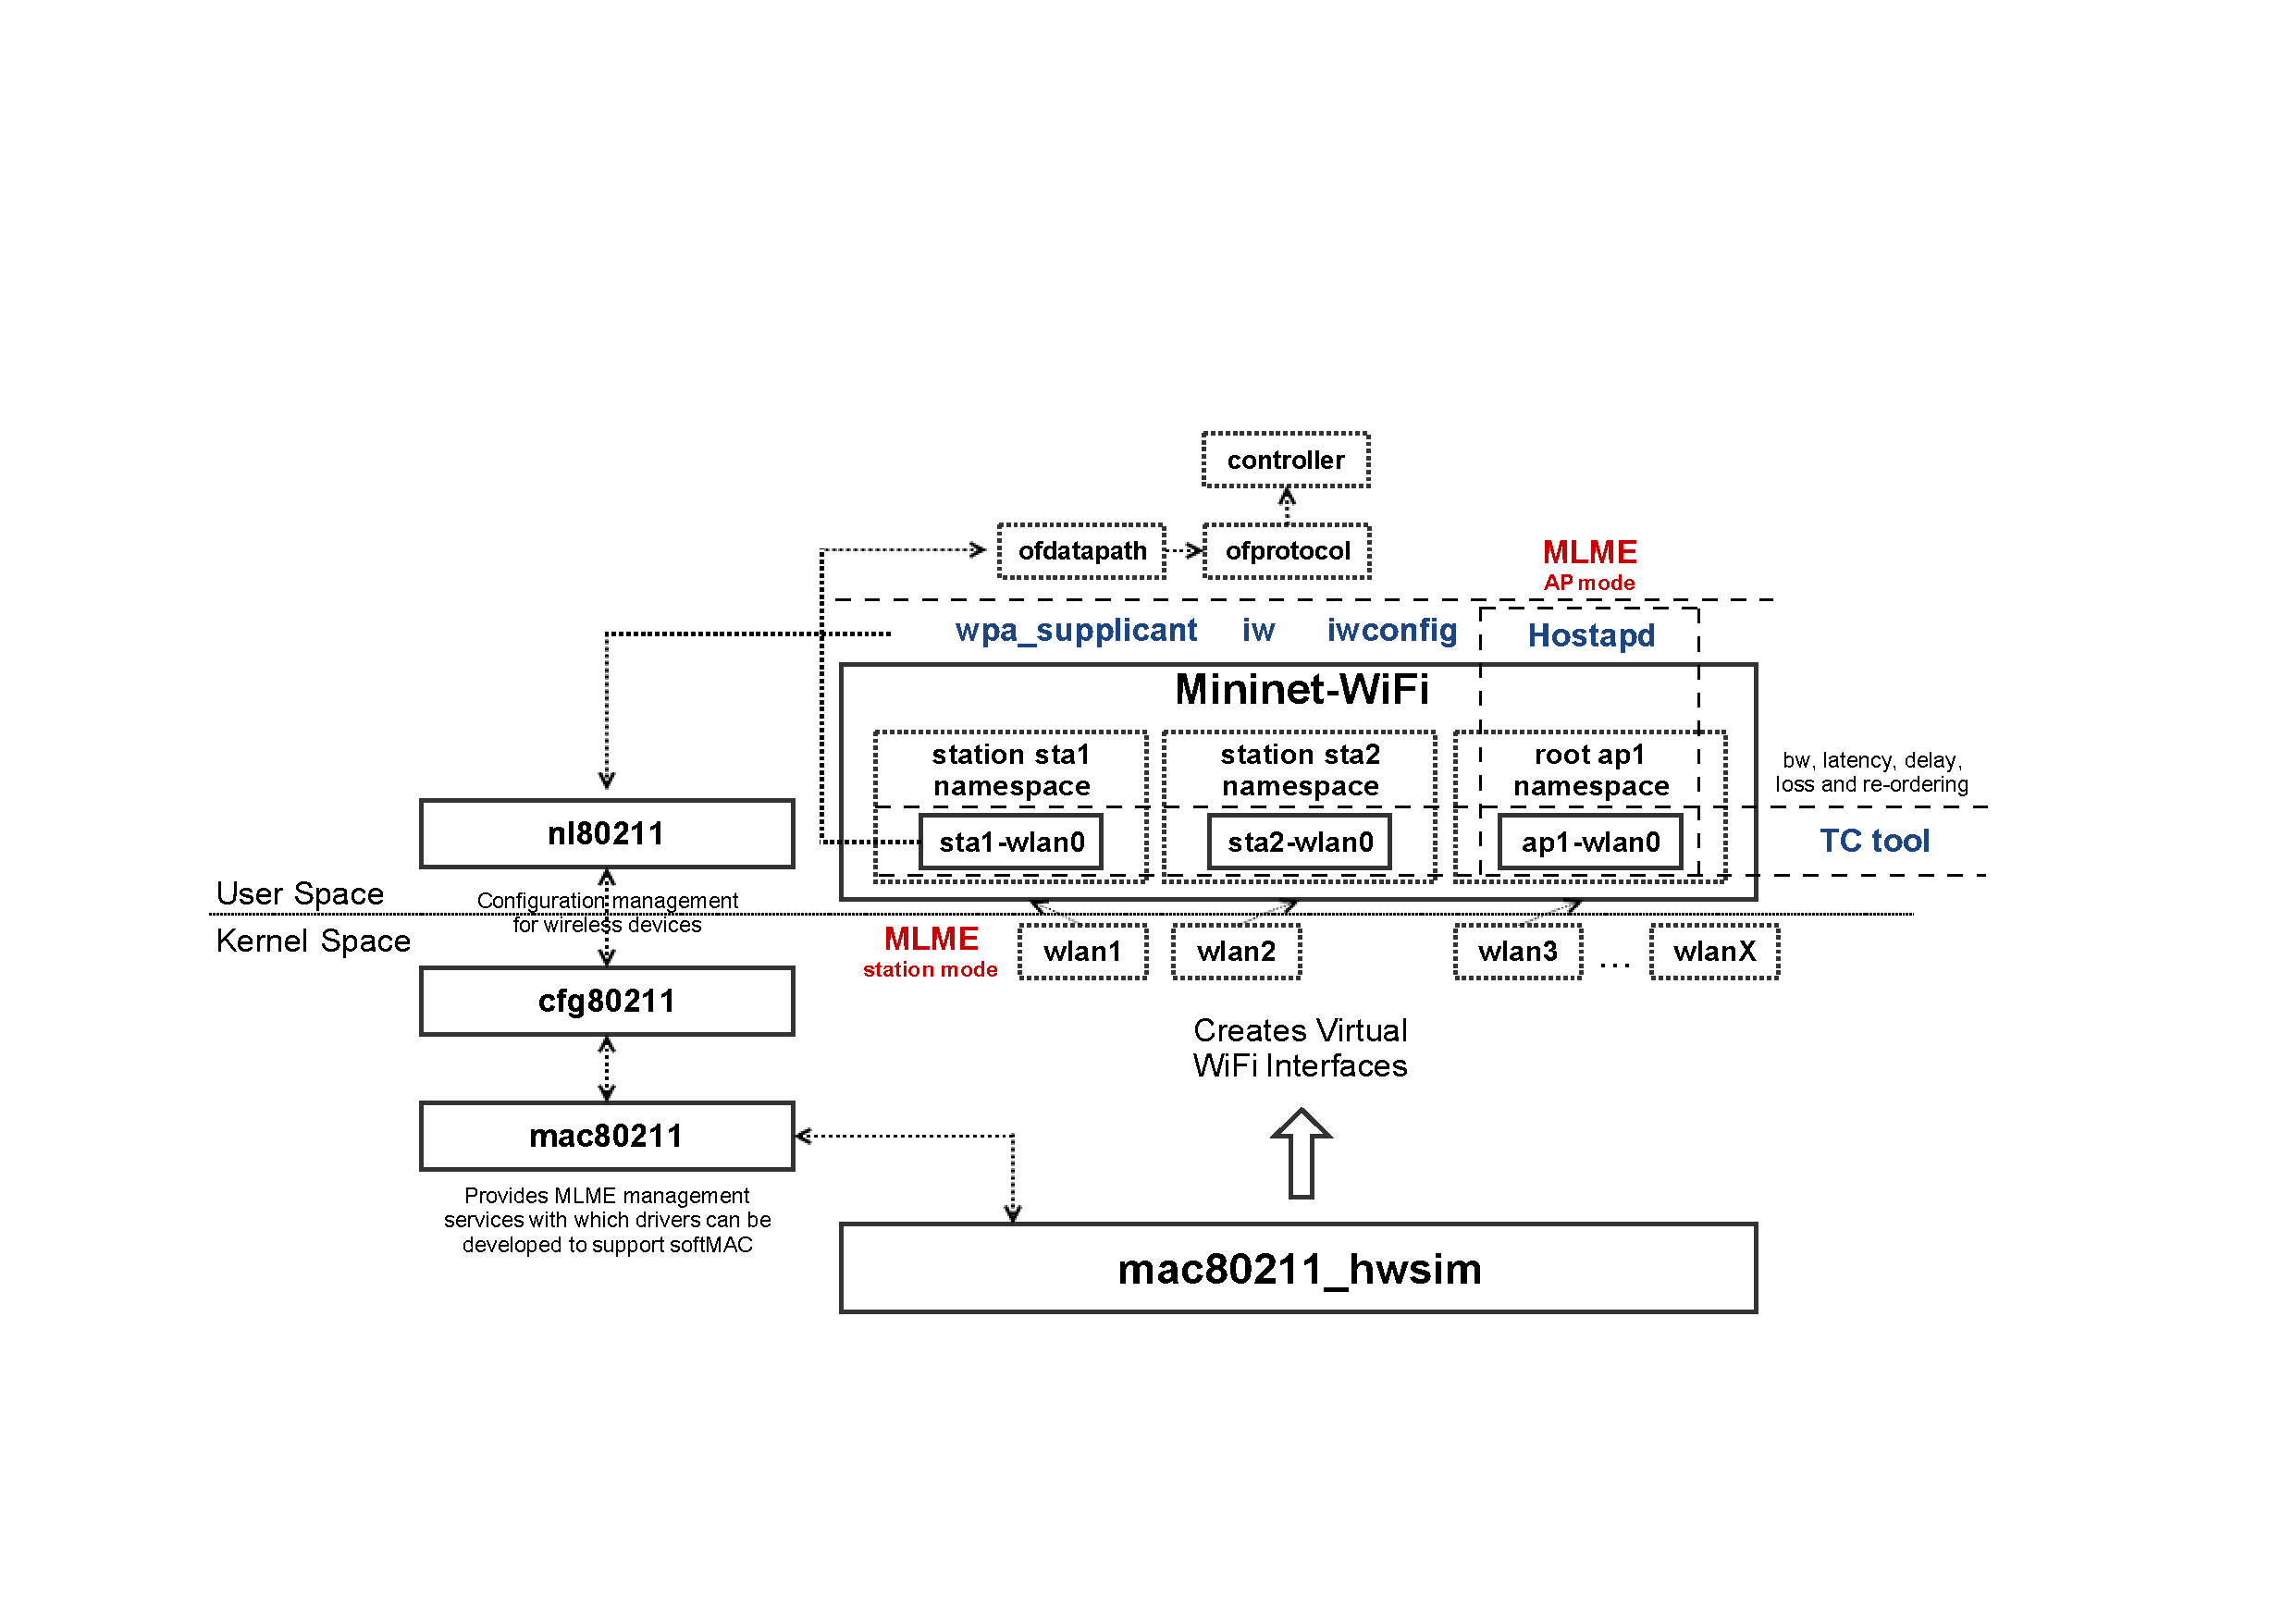
\includegraphics[trim=3.7cm 5cm 2.1cm 7.8cm,clip,width=1.1\textwidth]{Pictures/components}}
  \caption{Mininet-WiFi Components.}
   \label{flowchart}
\end{figure}

\begin{figure}[!t]
\centering
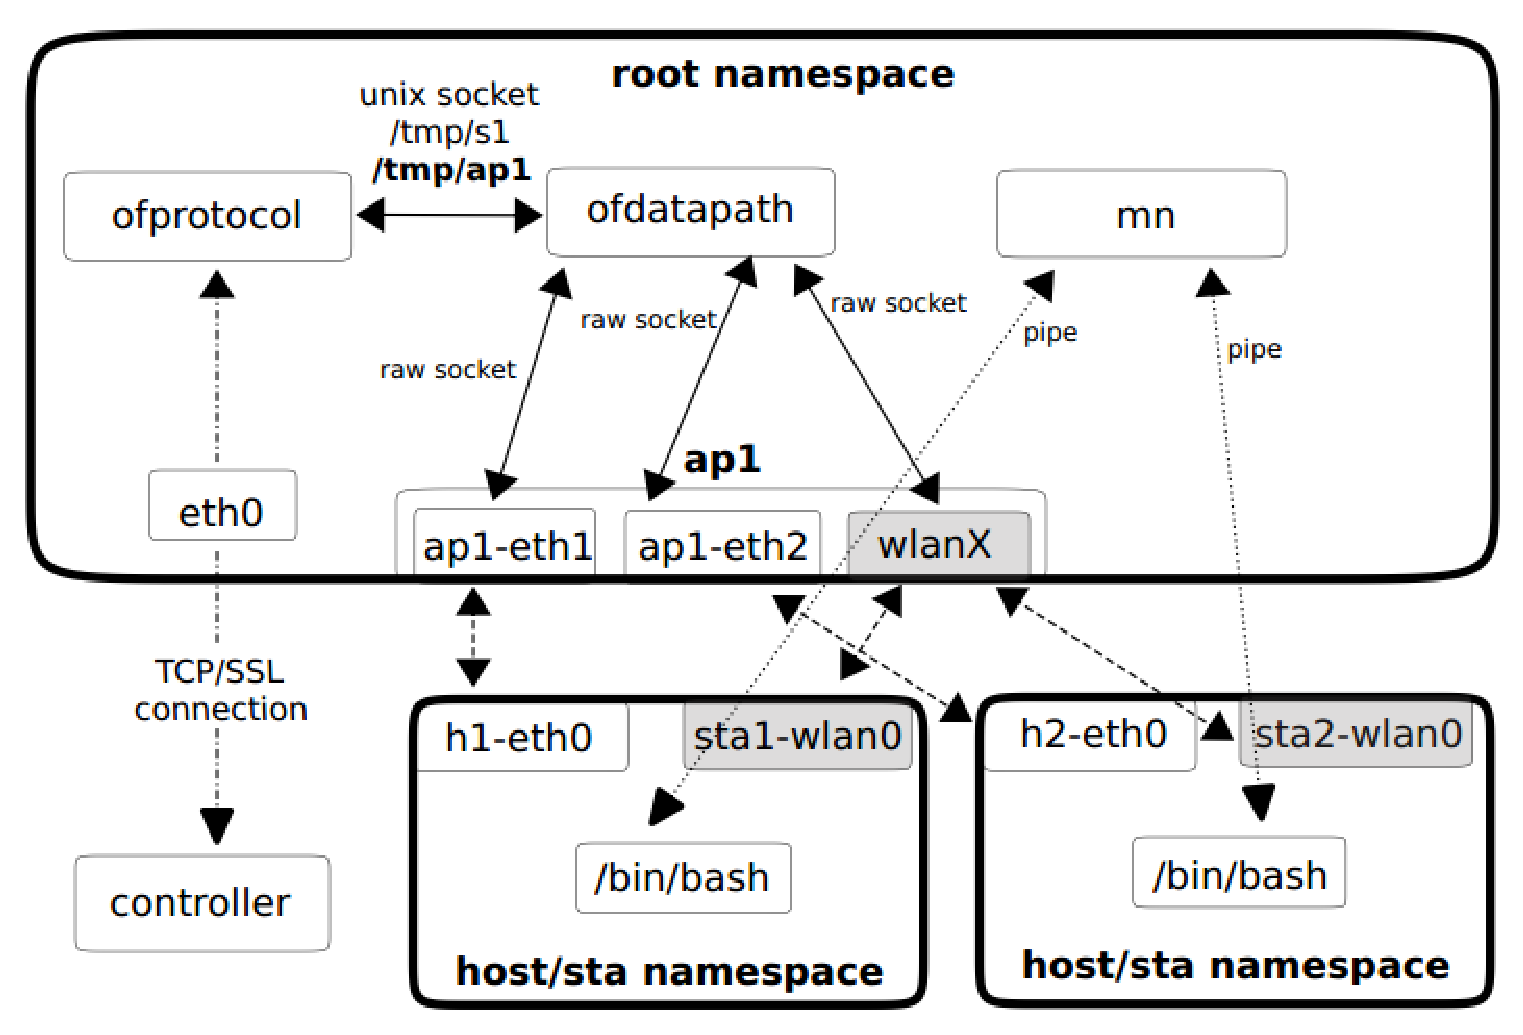
\includegraphics[width=0.7\textwidth]{Pictures/arch.eps}
\caption{Components and connections in a two-host network created with Mininet-WiFi.}
\label{fig:arch}
\end{figure}

Figure~\ref{fig:arch} depicts the components and connections in a simple topology with two stations (or hosts) created with Mininet-WiFi, where the newly implemented components (highlighted in gray) are presented along the original Mininet building blocks. Although stations are equipped with a wireless interface by default they are able to connect with access points through wired links (veth pairs) as well.  

More specifically, we added WiFi interfaces on stations that now are able to connect to an access point through its (\texttt{wlanX}) interface that is bridged to an OpenFlow switch with AP capabilities represented by (\texttt{ap1}). 
Similar to Mininet, the virtual network is created by placing host processes in Linux OS network namespaces interconnected through virtual Ethernet (veth) pairs. The wireless interfaces to virtualize WiFi devices work on \textit{master} mode for access points and \textit{managed} mode for stations.

\noindent \textbf{Stations:} Are devices that connect to an access point through authentication and association. In our implementation, each station has one wireless card (\texttt{staX-wlan0} - where X shall be replaced by the number of each station). Since the traditional Mininet hosts are connected to an access point, stations are able to communicate with those hosts.

\noindent \textbf{Access Points:} Are devices that manage associated stations. Virtualized through \texttt{hostapd}\footnote{Hostapd (\textbf{H}ost \textbf{A}ccess \textbf{P}oint \textbf{D}aemon) user space software capable of turning normal wireless network interface cards into access points and authentication servers} daemon and use virtual wireless interfaces for access point and authentication servers. 
While virtualized access points do not have (yet) APIs allowing users to configure several parameters in the same fashion of a real one, the current implementation covers the most important features, for example ssid, channel, mode, password, cryptography, etc.

Both stations and access points use \texttt{cfg80211} to communicate with the wireless device driver, a Linux 802.11 configuration API that provides communication between stations and \texttt{mac80211}. This framework in turn communicates directly with the WiFi device driver through a \texttt{netlink} socket (or more specifically \texttt{nl80211}) that is used to configure the \texttt{cfg80211} device and for kernel-user-space communication as well.

\subsection{Files}

\begin{itemize}
\item mininet/wifiAdHocConnectivity.py - checking adhoc pairs
\item mininet/wifiAssociationControl.py - association Control techniques
\item mininet/wifiChannel.py - channel details
\item mininet/wifiDevices.py - specification of real devices
\item mininet/wifiMeshRouting.py - wireless mesh routing
\item mininet/wifiMobility.py - mobility parameters
\item mininet/wifiMobilityModels.py - mobility models
\item mininet/wifiModule.py - module 
\item mininet/wifiPlot.py - graphs
\item mininet/wifiPropagationModels.py - propagation models
\item mininet/wifiReplaying.py - replaying captured traces
\item mininet/vanet.py - VANET networks
\end{itemize}

\subsection{Classes}\index{classes}

\begin{itemize}
\item \textit{UserAP():} User-space AP
\item \textit{OVSAP():} Open vSwitch AP
\item \textit{addHost():} adds a host to a topology and returns the host name
\item \textit{addAccessPoint():} adds an access point to a topology and returns the access point name
\item \textit{addCar():} adds a car to a topology and returns the car name
\item \textit{addPhysicalBaseStation():} attach a physical usb interface to a virtual base station to a topology and returns the physical base station name
\item \textit{addStation():} adds a station to a topology and returns the station name
\item \textit{addSwitch():} adds a switch to a topology and returns the switch name
\item \textit{addWirelessMeshAP():} adds an ap with wireless interface working as wireless mesh to a topology and returns the switch name
\item \textit{addLink():} adds a bidirectional link to a topology (and returns a link key, but this is not important). Links in Mininet-WiFi are bidirectional unless noted otherwise.

\item \textit{plotGraph():} use this class if you want to plot graph.
\item \textit{startMobility:} useful when you want to use a mobility model.
\end{itemize}



\section{Creating Network}\index{creatingNetwork}

You can create a simple network (2 stations and 1 access point) with the following command:
\begin{minted}{bash}
    sudo mn --wifi
\end{minted}

\noindent The command above can be utilized with other parameters, like in:
\begin{minted}{bash}
    sudo mn --wifi --ssid=new_ssid --mode=g --channel=1
\end{minted}

\noindent You can also use just mn if you want to work only with Mininet instead of Mininet-WiFi.

\subsection{Changing Topology Size and Type}\index{topo}
The default topology is a single Access Point connected to two Stations. You could change this to a different topo with --topo and pass parameters for that topology’s creation. For example, to verify all-pairs ping connectivity with one Access Point and five Stations:
\begin{minted}{bash}
    sudo mn --wifi --test pingall --topo single,5
\end{minted}

\noindent Another example, with a linear topology (where each Access Point has one station, and all Access Points connect in a line via wired media):
\begin{minted}{bash}
    sudo mn --wifi --test pingall --topo linear,5
\end{minted}

\subsection{Examples}\index{examples}
If you are just beginning to write scripts for Mininet-WiFi, you can use the example scripts as a starting point. We created example scripts in the \texttt{~/mininet-wifi/examples} directory that show how to use most of the features in Mininet-WiFi.

\subsection{Getting information}\index{gettinginfo}

\noindent \textit{getting the position:}
\begin{minted}{bash}
    mininet-wifi>py sta1.params['position']
\end{minted}

\noindent \textit{getting AP that a specific station is associated:}
\begin{minted}{bash}
    mininet-wifi>py sta1.params['associatedTo']
\end{minted}

\noindent \textit{getting APs in range:}
\begin{minted}{bash}
    mininet-wifi>py sta1.params['apsInRange']
\end{minted}

\noindent \textit{getting the channel:}
\begin{minted}{bash}
    mininet-wifi>py sta1.params['channel']
\end{minted}

\noindent \textit{getting the frequency:}
\begin{minted}{bash}
    mininet-wifi>py sta1.params['frequency']
\end{minted}

\noindent \textit{getting the mode:}
\begin{minted}{bash}
    mininet-wifi>py sta1.params['mode']
\end{minted}

\noindent \textit{getting the rssi:}
\begin{minted}{bash}
    mininet-wifi>py sta1.params['rssi']
\end{minted}

\noindent \textit{getting the Tx Power:}
\begin{minted}{bash}
    mininet-wifi>py sta1.params['txpower']
\end{minted}

\noindent \textit{getting associated stations to ap1:}
\begin{minted}{bash}
    mininet-wifi>py ap1.params['associatedStations']
\end{minted}

\subsection{Saving information}\index{saveinginfo}

You might want to save node parameters to a text file. To do so set \textbf{recordNodeParams} as True, for example:
\begin{minted}{bash}
    ap1 = net.addAccessPoint('ap1', recordNodeParams=True)
\end{minted}

\subsection{Changes at runtime}\index{changeatruntime}

\noindent \textit{setting the position:}
\begin{minted}{bash}
    mininet-wifi>py sta1.moveNodeTo('40,20,40')
\end{minted}

\noindent \textit{setting up the antenna gain:}
\begin{minted}{bash}
    mininet-wifi>py sta1.setAntennaGain('sta1-wlan0', 5)
\end{minted}

\noindent \textit{setting the signal range:}
\begin{minted}{bash}
    mininet-wifi>py sta.setRange(100)
\end{minted}

\noindent \textit{setting Tx Power:}
\begin{minted}{bash}
    mininet-wifi>py sta1.setTxPower('sta1-wlan0', 10)
\end{minted}

\noindent \textit{moving association to ap1:}
\begin{minted}{bash}
    mininet-wifi>py sta1.moveAssociationTo('sta1-wlan0', ap1)
\end{minted}

\section{Supported Features}

\subsection{Encryption}\index{encryption}
Mininet-WiFi supports WEP (Wired Equivalent Privacy), WPA (Wi-Fi Protected Access) and WPA2.

\subsubsection{Static WEP key configuration}
The key length should be 5, 13, or 16 characters (for ASCII WEP key), or 10, 26, or 32 digits (for hex WEP key), depending on whether 40-bit (64-bit), 104-bit (128-bit), or 128-bit (152-bit) WEP is used.

\subsection{Support to IEEE 802.11r}\index{80211r}

The example below enables 802.11r.

\begin{minted}[breaklines]{bash}
    ap1 = net.addAccessPoint( 'ap1', ssid="simplewifi", mode="g", channel="6", passwd='123456789a', encrypt='wpa2', ieee80211r='yes', mobility_domain='a1b2'
\end{minted}

\subsection{Support to bgscan (Background scanning)}\index{bgscan}

\texttt{wpa\_supplicant} behavior for background scanning can be specified by configuring a bgscan module. These modules are responsible for requesting background scans for the purpose of roaming within an ESS (i.e., within a single network block with all the APs using the same SSID). You can enable bgscan calling setBgscan(), for example:

\begin{minted}[breaklines]{bash}
    net.setBgscan()
\end{minted}
or
\begin{minted}[breaklines]{bash}
    net.setBgscan(module="$module_name", s_inverval=$value, signal=$value, l_interval=$value, database=$dir)
\end{minted}


\noindent s\_interval: \textit{short bgscan interval in seconds} \\
signal: \textit{signal strength threshold} \\
l\_interval: \textit{long interval} \\
database: \textit{<database file name>}

\noindent source: \url{https://w1.fi/cgit/hostap/plain/wpa_supplicant/wpa_supplicant.conf}

\subsection{Interference}\index{interference}
Mininet-WiFi supports the interference model provided by wmediumd. An example about how to enable interference is given below.

\begin{minted}[breaklines]{bash}
    net = Mininet( ... useWmediumd=True, enable_interference=True )
\end{minted}

The interference model implemented in wmediumd relies on CCA THRESHOLD (Clear Channel Assessment). The CCA is used by the MAC layer to determine (i) if the channel is clear for transmitting data, and (ii) for determining when there is incoming data. Evaluation of CCA is made by the PHY layer and the resulting assessment is communicated to the MAC layer via the PHY-CCA.indicate service primitive. This primitive can either be set to IDLE, when the channel is assessed to be clear, or BUSY when the channel is assessed to be in use.

%\textit{Wmediumd's rate table is currently hardcoded to IEEE 802.11a OFDM rates. Therefore, either operate wmediumd networks in 5 GHz channels, or supply a rateset for the BSS with no CCK rates.}

\subsection{Multiple SSIDs over a single AP}\index{multiplessid}
An unique AP supports up to 8 different SSIDs. You can configure multiple SSIDs separating different ssids by commas when you add an AP. For example:

\begin{minted}[breaklines]{bash}
    ap1 = net.addAccessPoint( 'ap1', ssid="ssid1,ssid2,ssid3", mode="g", channel="1" )
\end{minted}

\subsection{Support to WDS}\index{wds}
Wireless Distribution System (WDS) is supported by Mininet-WiFi with minor changes in mac80211\_hwsim. Further details about how to do these changes are available at \url{https://www.youtube.com/watch?v=a27qWHO8JDM}

\subsection{Including RSSI in the packet header}\index{rssi}
Although beacons can be captured using any packet sniffer, changes on the RSSI by the propagation models in place are
not included in the packet header by default. Minor changes are required in mac80211\_hwsim in order to fix this issue. Further details are available at: \url{https://www.youtube.com/watch?v=gtaHCpaHBGc}

\subsection{Support to Virtual Interfaces}\index{vifs}

The mac80211 subsystem in the linux kernel supports multiple wireless interfaces to be created with one physical wireless card. To do so you have to set the number of virtual interfaces to be created (nvif), as illustrated below.

\begin{minted}[breaklines]{bash}
    sta1 = net.addStation( 'sta1', nvif=2 )
\end{minted}

\subsection{Customizing Equations}\index{equation}
When a node is moving different values for bandwidth, latency, loss and delay are applied based on equations. Those equations can be customized by calling setChannelEquation(), for example:

\begin{minted}[breaklines]{bash}
#dist = distance between receiver and transmitter
#custombw = is a default value for bw which takes into account the RSSI
    net.setChannelEquation(bw='value.rate * (1.1 ** -dist)', loss='(dist * 2) / 100', delay='(dist / 10) + 1', latency='2 + dist')
\end{minted}

\subsection{Integration with Intermediate Functional Block (IFB) Devices}\index{ifb}\label{ifb}

Intermediate Functional Block (IFB) is an alternative to tc filters for handling ingress traffic, by redirecting it to a virtual interface and treat is as egress traffic. IFB is supported by calling net.useIFB() just after adding all nodes and before calling net.configureWifiNodes().
\\
Further information about IFB is available at \url{http://shorewall.net/traffic\_shaping.htm\#IFB}.



\subsection{Integration with wmediumd}\index{wmediumd}\label{wmediumd}
The kernel module mac80211\_hwsim uses the same virtual medium for all wireless nodes. This means all nodes are internally in range of each other and they can be discovered in a wireless scan on the virtual interfaces. Mininet-WiFi simulates their position and wireless ranges by assigning stations to other stations or access points and revoking these wireless associations. If wireless interfaces should be isolated from each other (e.g. in adhoc or mesh networks) a tool like \underline{\href{https://github.com/bcopeland/wmediumd}{wmediumd}}\footnote{https://github.com/bcopeland/wmediumd} is required. It uses a kind of a dispatcher to permit or deny the transfer of packets from one interface to another.\\
\\
Mininet-WiFi contains a small helper that should support when using wmediumd. It is located in \texttt{wmediumdConnector.py}. Two modes can be used when using this connector: dynamic and static mode.

\subsubsection{Dynamic mode}
This mode should be the best choice in most use cases. It requires the input of Mininet interfaces as Python objects and retrieves the MAC addresses which are required for wmediumd automatically from the Mininet API.\\
%\textbf{Please have in mind:} Even though it is called dynamic mode it does not mean that changes to the MAC addresses will be directed to wmediumd. Once it is initialized the configuration cannot be changed anymore which implies this is not suitable for mobility and manual position or range changes etc.\\
\\
At first you have to enter the connection properties for wmediumd. The following code snippet would create a linear topology in which sta1 can reach sta2, sta2 can reach sta3 (and vice versa) but sta1 can't reach sta3 directly.
\begin{minted}[breaklines]{bash}
sta1wlan0 = DynamicWmediumdIntfRef(sta1)
sta2wlan0 = DynamicWmediumdIntfRef(sta2)
sta3wlan0 = DynamicWmediumdIntfRef(sta3)

intfrefs = [sta1wlan0, sta2wlan0, sta3wlan0]
links = [
  WmediumdLink(sta1wlan0, sta2wlan0, 15),
  WmediumdLink(sta2wlan0, sta1wlan0, 15),
  WmediumdLink(sta2wlan0, sta3wlan0, 15),
  WmediumdLink(sta3wlan0, sta2wlan0, 15)]
WmediumdConn.set_wmediumd_data(intfrefs, links)
\end{minted}
The variables \texttt{staX-wlan0} are references to interfaces of Mininet-WiFi stations. If only the station is provided in the constructor, the default interface will be used. Other interfaces can be specified by adding an extra parameter containing the name of the interface.\\
The variable \texttt{intfrefs} has to contain all interfaces that should be monitored by wmediumd. If an interface is present in the link list, but not in the \texttt{intfrefs} list, an exception will be raised.\\
\texttt{links} has to contain all pairs of interfaces that should be able to reach the other one. Note: this can be asymmetrical, for example packets from sta1wlan0 could reach sta2wlan0 but not vice versa. If you want the connections to be symmetrical both pairs have to be present. The third parameter is the signal-noise-ratio which is used by wmediumd to simulate packet loss. Packet loss depends on the packet size and TX rate.\\
\\
If the Mininet-WiFi network is already started use the following method to start wmediumd:
\begin{minted}[breaklines]{bash}
WmediumdConn.connect_wmediumd_after_startup()
\end{minted}
%An example is located in \texttt{examples/wmediumd\_ibss\_dynamic.py}.\\
%\\
This has the disadvantage that some tools like \texttt{iw} use a cache and the stations previously discovered may appear even if they cannot be reached anymore.\\
To prevent this you can use another method:
\begin{minted}[breaklines]{bash}
WmediumdConn.connect_wmediumd_on_startup()
\end{minted}
This will hook into Mininet-WiFi and will start wmediumd right after the mac80211\_hwsim module is initialized. The method has to be called between the creation of stations (because the station objects are required) and before the net is started or any wireless associations are done.\\
\\
An example is located in \texttt{examples/wmediumd\_ibss\_dynamic\_intercept.py}.
\\
Consider to take examples/wmediumd\_mobility.py as example if you want to work with mobility.

\subsubsection{Static mode}
The static mode uses the MAC addresses that have been provided. In most cases the dynamic mode is the one to use. The advantage of the static mode is that no station objects are required and the data could be provided prior to the start of Mininet-WiFi.
\begin{minted}[breaklines]{bash}
sta1wlan0 = StaticWmediumdIntfRef('sta1', 'sta1-wlan0', '02:00:00:00:00:00')
sta2wlan0 = StaticWmediumdIntfRef('sta2', 'sta2-wlan0', '02:00:00:00:01:00')
sta3wlan0 = StaticWmediumdIntfRef('sta3', 'sta3-wlan0', '02:00:00:00:02:00')

intfrefs = [sta1wlan0, sta2wlan0, sta3wlan0]
links = [
  WmediumdLink(sta1wlan0, sta2wlan0, 15),
  WmediumdLink(sta2wlan0, sta1wlan0, 15),
  WmediumdLink(sta2wlan0, sta3wlan0, 15),
  WmediumdLink(sta3wlan0, sta2wlan0, 15)]
WmediumdConn.set_wmediumd_data(intfrefs, links)
\end{minted}
Station and interface names don't need to match real stations and real interfaces. They are just used to create an identifier that is used internally. The combination of station and interface name has to be unique.\\
\\
After the data is set, wmediumd can be started just like in dynamic mode.\\
\\
An example is located in \texttt{examples/wmediumd\_ibss\_static.py}.

\subsubsection{Installation of wmediumd}
It is required that wmediumd can be called using the command \texttt{wmediumd}. That means it should be located in \texttt{/usr/bin} or any other path that is available through the PATH enviroment variable.\\
wmediumd can be automatically installed using the \texttt{-l} option on \texttt{util/install.sh}. This will copy the binary to \texttt{/usr/bin/wmediumd}.


%\section{Known Issues}\index{issues}

%\subsection{WiFi-Direct}
%Working with wifidirect requires modification in wpa\_supplicant. You have to follow the steps described below in order to enable it:

%\begin{minted}{bash}
%cd wpa_supplicant/
%//Open defconfig and uncomment CONFIG_P2P=y
%//Save the file
%sudo cp defconfig .config
%//Open p2p_supplicant.c and search for:
%//define P2P_MGMT_DEVICE_PREFIX          "p2p-dev-"
%//and change it to
%//define P2P_MGMT_DEVICE_PREFIX          "p2p-"
%//Save the file
%sudo make install
%\end{minted}
%*We have faced troubles when \textit{wifi-direct} is enabled, cause it affects %scenarios that require wep and wpa. That's why it is not enabled by default.

\section{Videos}\index{videos}
You can find many videos about Mininet-WiFi in a \underline{\href{https://www.youtube.com/playlist?list=PLccoFREVAt\_4nEtrkl59mjjf5ZzRX8DZA}{channel on youtube}}\footnote{https://www.youtube.com/playlist?list=PLccoFREVAt\_4nEtrkl59mjjf5ZzRX8DZA}.

\section{Contact Us}\index{contact}
You are invited to participate of our \underline{\href{https://groups.google.com/forum/\#!forum/mininet-wifi-discuss}{mailing list}}\footnote{https://groups.google.com/forum/\#!forum/mininet-wifi-discuss}.


\section{FAQ}\index{faq}

\begin{itemize}
\item \textit{Question:} \textit{I am getting the following Error message:} \textbf{IndexError: list index out of range}. \textit{How to solve it?}\\
\textit{Answer:}
\begin{minted}{bash}
    sudo mn -c
\end{minted}
\item \textit{Question:} Is it possible to create a wired link between station and ap?\\
\textit{Answer:} Yes. When you add a link between station and ap you have to add the parameter link='wired' (e.g. net.addLink(sta1, ap2, link='wired')\\

\item \textit{May I customize the Access Point and Station configuration file?}
\\
\textit{Answer:} Since the Access Point is based on Hostapd you may customize the configuration file generated by Mininet-WiFi adding the parameter \texttt{config} when you create the access point, for example:\\

\begin{minted}[breaklines]{bash}
    ap1 = net.addAccessPoint( 'ap1', config='ctrl_interface=/var/run/hostapd/,ctrl_interface_group=0' )
\end{minted}

The code above will create the file ap1-wlan1.apconf. \\

The same can be done for stations when wpa\_supplicant is used, for example:

\begin{minted}[breaklines]{bash}
    sta1 = net.addStation( 'sta1', config='eap=PEAP,identity="bob"' )
\end{minted}


\item \textit{Is it possible to plot hosts in graph?}
Yes, it is possible. You have to call the method below before creating any link between two nodes with addLink():

\begin{minted}[breaklines]{bash}
    net.plotNode(h1, position='10,10,0')
\end{minted}
\end{itemize}
\chapterimage{logo.png}
\chapter{Mobility Models}

\section{Mobility Models Supported}
Mininet-WiFi supports the following mobility models: \texttt{RandomWalk}, \texttt{TruncatedLevyWalk}, \texttt{RandomDirection}, \texttt{RandomWayPoint}, \texttt{GaussMarkov}, \texttt{ReferencePoint} and \texttt{TimeVariantCommunity}.

\section{How to add Mobility?}
To use those mobility models you have to call the method net.startMobility() like in \textit{examples/wifiMobilityModel.py}. You may also have to consider the use of the files \textit{examples/wifiMobility.py} and \textit{examples/tracingMobility.py} if you want a different type of mobility. Another alternative is to consider some parameters for specifics mobility models (not mandatory), for example:

\subsubsection{RandomWalk}

\begin{minted}[breaklines]{bash}
sta1 = net.addStation( ..., min_x=10, max_x=20, min_y=10, max_y=20, constantDistance=1, constantVelocity=1 )

min_x = Minimum X position
max_x = Maximum X position
min_y = Minimum Y position
max_y = Maximum Y position
constantDistance = the value for the constant distance traveled in each step. Default is 1.0.
constantVelocity = the value for the constant node velocity. Default is 1.0
\end{minted}

\subsubsection{RandomDirection}

\begin{minted}[breaklines]{bash}
sta1 = net.addStation( ..., min_x=10, max_x=20, min_y=10, max_y=20, min_v=1, max_v=2 )

min_x = Minimum X position
max_x = Maximum X position
min_y = Minimum Y position
max_y = Maximum Y position
min_v = Minimum value for node velocity
max_v = Maximum value for node velocity
\end{minted}

\subsubsection{RandomWayPoint}

\begin{minted}[breaklines]{bash}
sta1 = net.addStation( ..., min_x=10, max_x=20, min_y=10, max_y=20, min_v=1, max_v=2 )
//min_v and max_v must have different values

min_x = Minimum X position
max_x = Maximum X position
min_y = Minimum Y position
max_y = Maximum Y position
min_v = Minimum value for node velocity
max_v = Maximum value for node velocity
\end{minted}

\subsubsection{GaussMarkov}

\begin{minted}[breaklines]{bash}
sta1 = net.addStation( ..., min_x=10, max_x=20, min_y=10, max_y=20 )

min_x = Minimum X position
max_x = Maximum X position
min_y = Minimum Y position
max_y = Maximum Y position

\end{minted}


\begin{remark}
Thank you Mark Zeng (n660123@gmail.com) for recommending us the limit of the node motion.
\end{remark}
\chapterimage{logo.png}
\chapter{Propagation Models}
\section{Propagation Models Supported}
Mininet-WiFi supports the following propagation models: \texttt{Friis Propagation Loss Model}, \texttt{Log-Distance Propagation Loss Model}, \texttt{Log-Normal Shadowing Propagation Loss Model}, \texttt{International Telecommunication Union (ITU) Propagation Loss Model} and \texttt{Two-Ray Ground Propagation Loss Model}.

\section{How to add specific Propagation Model?}
You have to call the method \texttt{net.propagationModel()} like in \textit{examples/propagationModel.py}. You might have to consider some parameters for specifics propagation models (not mandatory), for example:

\subsubsection{Friis Propagation Loss Model}
\begin{minted}{bash}
net.propagationModel("friisPropagationLossModel", sL = $int) 
sL = system loss
\end{minted}

\subsubsection{Log-Distance Propagation Loss Model}
\begin{minted}[breaklines]{bash}
net.propagationModel("logDistancePropagationLossModel", sL = $int, exp = $int) 
sL = system loss
exp = exponent
\end{minted}

\subsubsection{Log-Normal Shadowing Propagation Loss Model}
\begin{minted}[breaklines]{bash}
net.propagationModel("logNormalShadowingPropagationLossModel", sL = $int, exp = $int, gRandom = $int) 
sL = system loss
exp = exponent
gRandom = gaussian random variable
\end{minted}

\subsubsection{International Telecommunication Union (ITU) Propagation Loss Model}
\begin{minted}{bash}
net.propagationModel("ITUPropagationLossModel", lF = $int, nFloors = $int, pL = $int)  
lF = floor penetration loss factor
nFloors = number of floors
pL = power loss coefficient
\end{minted}

\subsubsection{Two-Ray Ground Propagation Loss Model}
\textit{Attention: It does not give a good result for a short distance}
\begin{minted}{bash}
net.propagationModel("twoRayGroundPropagationLossModel")	
\end{minted}
\chapterimage{logo.png}
\chapter{Replaying Traces}
\textbf{\textcolor{red}{Development still in progress}}

\section{Replaying Mobility}\index{repMobility}
See the file examples/replaying/replayingMobility.py

\section{Replaying Bandwidth}\index{repBandwidth}
See the file examples/replaying/replayingBandwidth.py

\section{Replaying RSSI}\index{repRSSI}
See the file examples/replaying/replayingRSSI.py
\chapterimage{logo.png}
\chapter{Tutorial}\label{tutorial}

\section{Introduction}\index{intro}
This tutorial has been developed by Brian Linkletter (http://www.brianlinkletter.com/mininet-wifi-software-defined-network-emulator-supports-wifi-networks). We thank Brian for his time and this helpful tutorial.

\section{First ideas}\index{First ideas}

In this post, I describe the unique functions available in the Mininet-WiFi network emulator and work through a few tutorials exploring its features.

\subsection{How to read this post}

In this post, I present the basic functionality of Mininet-WiFi by working through a series of tutorials, each of which works through Mininet-WiFi features, while building on the knowledge presented in the previous tutorial. I suggest new users work through each tutorial in order.

I do not attempt to cover every feature in Mininet-WiFi. Once you work through the tutorials in this post, you will be well equipped to discover all the features in Mininet-WiFi by working through the \texttt{Mininet-WiFi example scripts}- https://github.com/intrig-unicamp/mininet-wifi/tree/master/examples, and reading the \texttt{Mininet-WiFi wiki}\footnote{https://github.com/intrig-unicamp/mininet-wifi/wiki} and \texttt{mailing list}\footnote{https://groups.google.com/forum/\#!forum/mininet-wifi-discuss}.

I assume the reader is already familiar with the [Mininet network emulator](http://mininet.org/) so I cover only the new WiFi features added by Mininet-WiFi. If you are not familiar with Mininet, please read my \texttt{Mininet network simulator review}\footnote{http://www.brianlinkletter.com/mininet-test-drive/} before proceeding. I have also written \texttt{many other posts about Mininet}\footnote{http://www.brianlinkletter.com/tag/mininet/}.

I start by discussing the functionality that Mininet-WiFi adds to Mininet: Mobility functions and WiFi interfaces. Then I show how to install Mininet-WiFi and work through the tutorials listed below:

Tutorial \#1: One access point shows how to run the simplest Mininet-WiFi scenario, shows how to capture wireless traffic in a Mininet-Wifi network, and discusses the issues with OpenFlow and wireless LANs.

Tutorial \#2: Multiple access points shows how to create a more complex network topology so we can experiment with a very basic mobility scenario. It discusses more about OpenFlow and shows how the Mininet reference controller works in Mininet-WiFi.

Tutorial \#3: Python API and scripts shows how to create more complex network topologies using the Mininet-WiFi Python API to define node positions in space and other node attributes. It also discusses how to interact with nodes running in a scenario with the Mininet-WiFi CLI, the Mininet-WiFi Python interpreter, and by running commands in a node's shell.

Tutorial \#4: Mobility shows how to create a network mobility scenario in which stations move through space and may move in and out of range of access points. It also discusses the available functions that may be used to implement different mobility models using the Mininet-WiFi Python API.


\subsection{Mininet-WiFi compared to Mininet}

Mininet-WiFi is an extension of the Mininet software defined network emulator. The Mininet-WiFi developer did not modify any existing Mininet functionality, but added new functionality.

\subsection{Mininet-WiFi and Mobility}

Broadly defined, mobility in the context of data networking refers to the ability of a network to accommodate hosts moving from one part of the network to another. For example: a cell phone user may switch to a wifi access point when she walks into a coffee shop; or a laptop user may walk from her office in one part of a building to a meeting room in another part of the building and still being able to connect to the network via the nearest WiFi access point.

While the standard Mininet network emulator may be used to test mobility (In the Mininet examples folder, we find a \texttt{mobility.py} script that demonstrates methods that may be used to create a scenario where a host connected to one switch moves its connection to another switch), Mininet-WiFi offers more options to emulate complex scenarios where many hosts will be changing the switches to which they are connected. Mininet-WiFi adds new classes that simplify the programming work required by researchers to create Mobility scenarios.

Mininet-WiFi does not modify the reference SDN controller provided by standard Mininet so the reference controller cannot manage the mobility of users in the wireless network. Researchers must use a remote controller that supports the CAPWAP protocol (NOTE: I've not tried this and I do not know if it will work without modifications or additional programming), or manually add and delete flows in the access points and switches.

\subsection{802.11 Wireless LAN Emulation}

Mininet-wifi incorporates the Linux 802.11 SoftMAC\footnote{https://wireless.wiki.kernel.org/en/developers/documentation/glossary\#softmac} wireless drivers, the cfg80211\footnote{http://www.linuxwireless.org/en/developers/Documentation/cfg80211} wireless configuration interface and the mac80211\_hwsim\footnote{https://wireless.wiki.kernel.org/en/users/drivers/mac80211\_hwsim} wireless simulation drivers in its access points. 

The \texttt{mac80211\_hwsim} driver is a software simulator for Wi-Fi radios. It can be used to \texttt{create virtual wi-fi interfaces}\footnote{http://stackoverflow.com/questions/33091895/virtual-wifi-802-11-interface-similar-to-veth-on-linux} that use the \texttt{802.11 SoftMAC wireless LAN driver}\footnote{http://linuxwireless.org/en/developers/Documentation/mac80211/\_\_v49.html}. Using this tool, researchers may \texttt{emulate a Wi-Fi link between virtual machines}\footnote{https://w1.fi/cgit/hostap/plain/tests/hwsim/example-setup.txt} - some mac80211\_hwsim practical examples and supporting information are at the following links: \texttt{lab}\footnote{http://www2.cs.siu.edu/\~sharvey/code/cs441/cs441\_lab.pdf}, \texttt{thesis}\footnote{http://upcommons.upc.edu/bitstream/handle/2099.1/19202/memoria.pdf?sequence=4}, \texttt{hostapd}\footnote{https://nims11.wordpress.com/2012/04/27/hostapd-the-linux-way-to-create-virtual-wifi-access-point/}, \texttt{wpa-supplicant}\footnote{https://wiki.debian.org/WiFi/HowToUse\#wpa\_supplicant}, \texttt{docs-1}\footnote{https://www.kernel.org/doc/readme/Documentation-networking-mac80211\_hwsim-README}, and \texttt{docs-2}\footnote{https://github.com/penberg/linux-kvm/tree/master/Documentation/networking/mac80211\_hwsim))}. The 80211\_hwsim driver enables researchers to emulate the wifi protocol control messages passing between virtual wireless access points and virtual mobile stations in a network emulation scenario. By default, 80211\_hwsim simulates perfect conditions, which means there is no packet loss or corruption.

You can use Wireshark to \texttt{monitor wireless traffic}\footnote{http://sandilands.info/sgordon/capturing-wireless-lan-with-ubuntu-tcpdump-kismet} passing between the virtual wireless access point and the virtual mobile stations in the Mininet-wifi network scenarios. But, you will find it is difficult to capture wireless control traffic on standard WLAN interfaces like \texttt{ap1-wlan0} because the Linux kernel \texttt{strips wireless control messages and headers}\footnote{https://wiki.wireshark.org/Wi-Fi} before making traffic on these interfaces available to user processes like Wireshark. You will have to install additional tools and follow a complex procedure to \texttt{enable monitoring of WiFi traffic on the \texttt{ap1-wlan0} interface}\footnote{https://wiki.wireshark.org/CaptureSetup/WLAN\#Linux}. An easier method is available: look for the \texttt{hwsim0} interface on an access point, enable it, and monitor traffic on it. The \texttt{hwsim0} interface replays communications sent onto the access point's simulated wireless interface(s) such as \texttt{ap1-wlan0} without stripping any 802.11 headers or control traffic\footnote{from http://teampal.mc2lab.com/attachments/685/C2012-12.pdf}. We'll see this in the examples we work through, below.

\subsection{Mininet-WiFi display graph}

Since locations of nodes in space is an important aspect of WiFi networks, Mininet WiFi provides a graphical display (figure~\ref{fig:mngraph}) showing locations of WiFi nodes in a graph. The graph may be created by calling its method in the Mininet-WiFi Python API (see examples in the tutorials below).

\begin{figure}
    \centering
    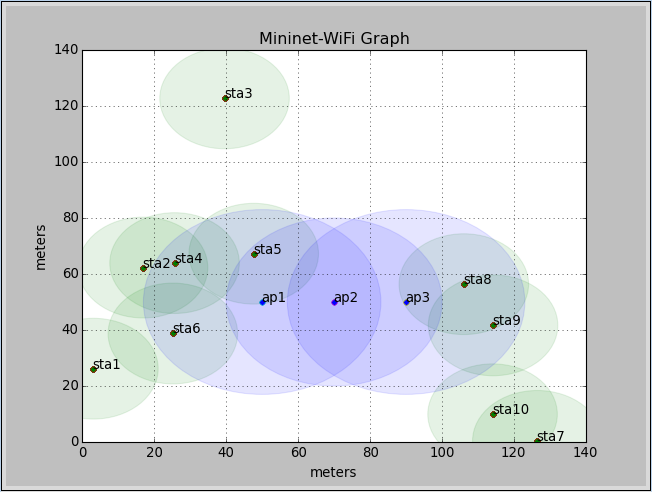
\includegraphics[width=0.7\textwidth]{Pictures/mn-wifi-graph-200}
    \caption{Mininet-WiFi Graph}
    \label{fig:mngraph}
\end{figure}

The graph will show wireless access points and stations, their positions in space and will display the affects of the range parameter for each node. The graph will not show any "wired" network elements such as standard Mininet hosts or switches, Ethernet connections between access points, hosts, or switches.

\subsection{Install Mininet-WiFi on a Virtual Machine}

First, we need to create a virtual machine that will run the Mininet-WiFi network emulator. In the example below, we will use the VirtualBox virtual machine manager because it is open-source and runs on Windows, Mac OS, and Linux.

\subsection{Set up a new Ubuntu Server VM}

Install Ubuntu Server in a new VM. Download an Ubuntu Server ISO image from the Ubuntu web site. See my post about \texttt{installing Debian Linux in a VM}\footnote{http://www.brianlinkletter.com/installing-debian-linux-in-a-virtualbox-virtual-machine/}. Follow the same steps to install Ubuntu.
\\
\\
In this example, we will name the VM \texttt{Mininet-WiFi}.

\subsection{Set up the Mininet-WiFi VM}

To ensure that the VM can display X applications such as Wireshark on your host computer's desktop, read through my post about \texttt{setting up the standard Mininet VM}\footnote{http://www.brianlinkletter.com/set-up-mininet/} and set up the host-only network adapter, the X windows server, and your SSH software.
\\
\\
Now you can connect to the VM via SSH with X Forwarding enabled. In the example below, my host computer is \texttt{t420} and the Mininet WiFi VM is named \texttt{wifi}.

\begin{minted}{bash}
t420:~$ ssh -X 192.168.52.101
wifi:~$
\end{minted}

\section{Mininet-WiFi Tutorial \#1: One access point}

The simplest network is the default topology, which consists of a wireless access point with two wireless stations. The access point is a switch connected to a controller. The stations are hosts.\\\\

\noindent This simple lab will allow us to demonstrate how to capture wireless control traffic and will demonstrate the way an OpenFlow-enabled access point handles WiFi traffic on the \texttt{wlan} interface.

\subsection{Capturing Wireless control traffic in Mininet-WiFi}

To view wireless control traffic we must first start Wireshark:

\begin{minted}{bash}
    wifi:~$ wireshark &
\end{minted}

\noindent Then, start Mininet-WiFi with the default network scenario using the command below:

\begin{minted}{bash}
    wifi:~$ sudo mn --wifi
\end{minted}

\noindent Next, enable the \texttt{hwsim0} interface. The \texttt{hwsim0} interface is the software interface created by Mininet-WiFi that copies all wireless traffic to all the virtual wireless interfaces in the network scenario. It is the easiest way to monitor the wireless packets in Mininet-WiFi.

\begin{minted}{bash}
    mininet-wifi> sh ifconfig hwsim0 up
\end{minted}

\noindent Now, in Wireshark (figure~\ref{fig:capture}, refresh the interfaces and then start capturing packets on the *hwsim0* interface. You should see wireless control traffic. Next, run a \texttt{ping} command:

\begin{minted}{bash}
    mininet-wifi> sta1 ping sta2
\end{minted}    

\begin{figure}
    \centering
    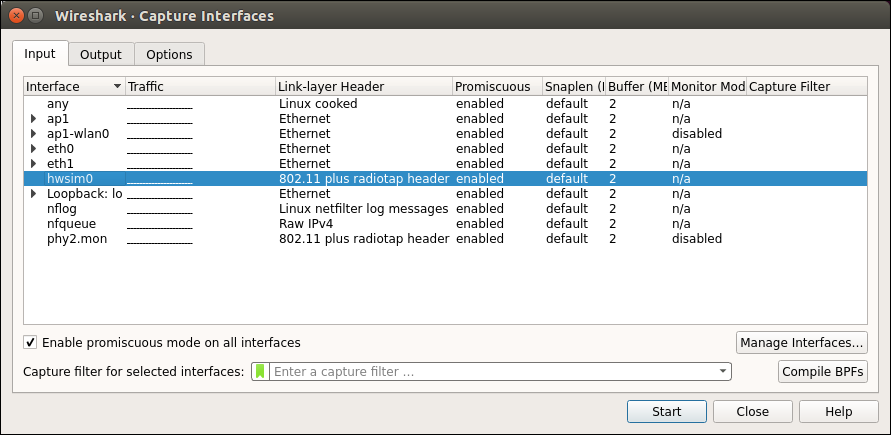
\includegraphics[width=0.7\textwidth]{Pictures/mn-wifi-008.png}
    \caption{Start capture on hwsim0 interface}
    \label{fig:capture}
\end{figure}

\noindent In Wireshark (figure~\ref{fig:traffic-wireshark}), see the wireless frames and the ICMP packets encapsulated in Wireless frames passing through the \texttt{hwsim0} interface. Stop the ping command by pressing \texttt{Ctrl-C}. In this default setup, any flows created in the access point (that's if they're created -- see below for more on this issue) will expire in 60 seconds.


\begin{figure}
    \centering
    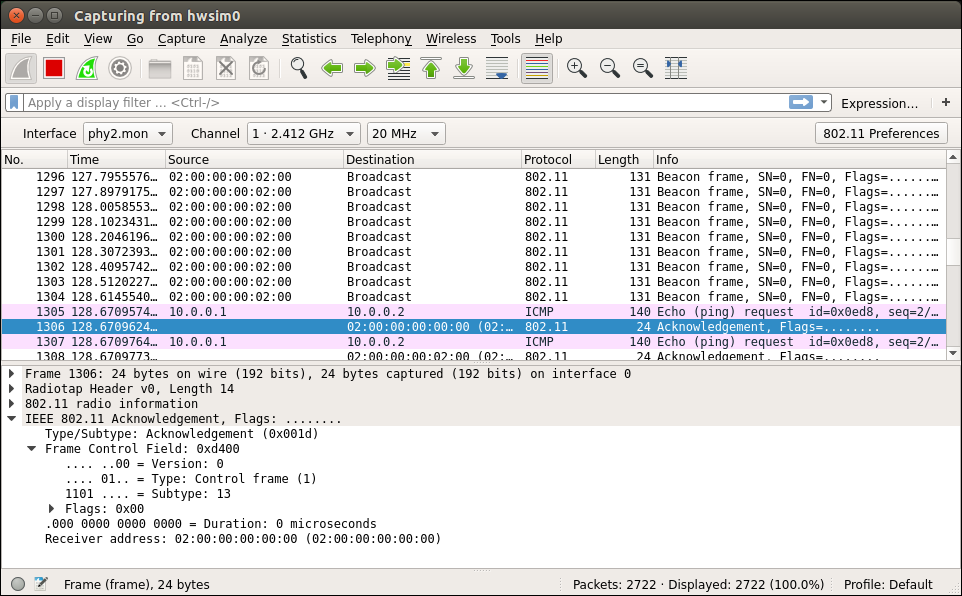
\includegraphics[width=0.7\textwidth]{Pictures/mn-wifi-010.png}
    \caption{Wireshark capturing WiFi control traffic}
    \label{fig:traffic-wireshark}
\end{figure}

\subsection{Wireless Access Points and OpenFlow}

In this simple scenario, the access point has only one interface, \texttt{ap1-wlan0}. By default, stations associated with an access point connect in \texttt{infrastructure mode} so wireless traffic between stations must pass through the access point. If the access point works similarly to a switch in standard Mininet, we expect to see OpenFlow messages exchanged between the access point and the controller whenever the access point sees traffic for which it does not already have flows established.

To view OpenFlow packets, stop the Wireshark capture and switch to the \texttt{loopback} interface. Start capturing again on the \texttt{loopback interface}. Use the \texttt{OpenFlow\_1.0} filter to view only OpenFlow messages.
\\
\\
\noindent Then, start some traffic running with the \texttt{ping} command and look at the OpenFlow messages captured in Wireshark.

\begin{minted}{bash}
    mininet-wifi> sta1 ping sta2
\end{minted}   

I was expecting that the first ICMP packet generated by the \texttt{ping} command should be flooded to the controller, and the controller would set up a flows on the access point so the two stations could exchange packets. Instead, I found that the two stations were able to exchange packets immediately and the access point did not flood the ICMP packets to the controller. Only an ARP packet, which is in a broadcast frame, gets flooded to the controller and is ignored (figure~\ref{fig:ofmsg}. \\

\begin{figure}
    \centering
    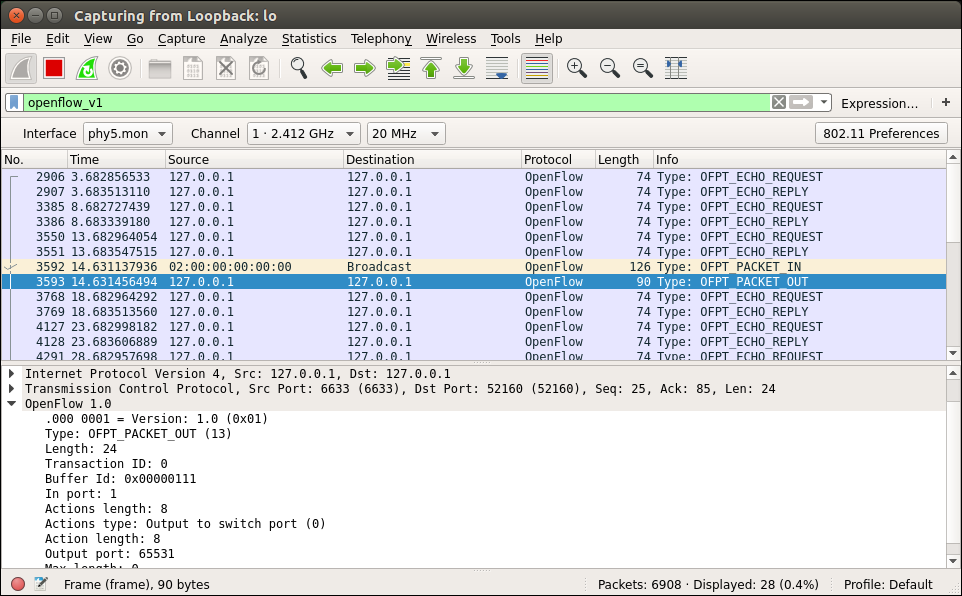
\includegraphics[width=0.7\textwidth]{Pictures/mn-wifi-20.png}
    \caption{No OpenFlow messages passing to the controller}
    \label{fig:ofmsg}
\end{figure}

\noindent Check to see if flows have been created in the access point:

\begin{minted}{bash}
    mininet-wifi> dpctl dump-flows
    *** ap1 ------------------------------------------
    NXST_FLOW reply (xid=0x4):
\end{minted}   

We see that no flows have been created on the access point. How do the two access points communicate with each other?

I do not know the answer but I have an idea. My research indicates that OpenFlow-enabled switches (using OpenFlow 1.0 or 1.3) will reject "hairpin connections", which are flows that cause traffic to be sent out the same port in which it was received. A wireless access point, by design, receives and sends packets on the same wireless interface. Stations connected to the same wireless access point would require a "hairpin connection" on the access point to communicate with each other. I surmise that, to handle this issue, Linux treats the WLAN interface in each access point like the radio network sta1-ap1-sta2 as if it is a "hub", where \texttt{ap1-wlan0} provides the "hub" functionality for data passing between sta1 and sta2. \texttt{ap1-wlan0} switches packets in the wireless domain and will not bring a packet into the "Ethernet switch" part of access point \texttt{ap1} unless it must be switched to another interface on \texttt{ap1} other than back out \texttt{ap1-wlan0}.

\subsection{Stop the tutorial}

Stop the Mininet \texttt{ping} command by pressing \texttt{Ctrl-C}. 

\noindent In the Wireshark window, stop capturing and quit Wireshark.

\noindent Stop Mininet-Wifi and clean up the system with the following commands:

\begin{minted}{bash}
    mininet-wifi> exit
    wifi:~$ sudo mn -c
\end{minted}
    
\section{Mininet-WiFi Tutorial \#2: Multiple access points}

When we create a network scenario with two or more wireless access points, we can show more of the functions available in Mininet-WiFi. 

In this tutorial, we will create a linear topology with three access points, where one station is connected to each access point. Remember, you need to already know \texttt{basic Mininet commands}\footnote{http://mininet.org/walkthrough/} to appreciate how we create topologies using the Mininet command line. 

Run Mininet-Wifi and create a linear topology with three access points:

\begin{minted}{bash}
    sudo mn --wifi --topo linear,3
\end{minted}
    
From the output of the command, we can see how the network is set up and which stations are associated with which access points.

\begin{minted}{bash}
*** Creating network
*** Adding controller
*** Adding hosts and stations:
sta1 sta2 sta3
*** Adding switches and access point(s):
ap1 ap2 ap3
*** Adding links and associating station(s):
(ap2, ap1) (ap3, ap2) (sta1, ap1) (sta2, ap2) (sta3, ap3)
*** Starting controller(s)
c0
*** Starting switches and access points
ap1 ap2 ap3 ...
*** Starting CLI:
mininet-wifi>
\end{minted}
    
We can also verify the configuration using the Mininet CLI commands \texttt{net} and \texttt{dump}. For example, we can run the \texttt{net} command to see the connections between nodes:

\begin{minted}{bash}
mininet-wifi> net
sta1 sta1-wlan0:None
sta2 sta2-wlan0:None
sta3 sta3-wlan0:None
ap1 lo:  ap1-eth1:ap2-eth1
ap2 lo:  ap2-eth1:ap1-eth1 ap2-eth2:ap3-eth1
ap3 lo:  ap3-eth1:ap2-eth2
c0
\end{minted}
    
From the \texttt{net} command above, we see that ap1, ap2, and ap3 are connected together in a linear fashion by Ethernet links. But, we do not see any information about to which access point each station is connect. This is because they are connected over a "radio" interface so we need to run the \texttt{iw} command at each station to observe to which access point each is associated.

To check which access points are "visible" to each station, use the \texttt{iw scan} command:

\begin{minted}{bash}
mininet-wifi> sta1 iw dev sta1-wlan0 scan | grep ssid
    SSID: ssid_ap1
    SSID: ssid_ap2
    SSID: ssid_ap3
\end{minted}

Verify the access point to which each station is currently connected with the \texttt{iw link} command. For example, to see the access point to which station \texttt{sta1} is connected, use the following command:

\begin{minted}{bash}
mininet-wifi> sta1 iw dev sta1-wlan0 link
    Connected to 02:00:00:00:03:00 (on sta1-wlan0)
            SSID: ssid_ap1
            freq: 2412
            RX: 1853238 bytes (33672 packets)
            TX: 7871 bytes (174 packets)
            signal: -30 dBm
            tx bitrate: 54.0 MBit/s
           
            bss flags:      short-slot-time
            dtim period:    2
            beacon int:     100
mininet-wifi>
\end{minted}
    

\subsection{A simple mobility scenario}

In this example, each station is connected to a different wireless access point. We can use the \texttt{iw} command to change which access point to which each station is connected. 

Note: The \texttt{iw} commands may be used in static scenarios like this but should not be used when Mininet-WiFi automatically assigns associations in more realistic mobility scenarios. We’ll discuss how Mininet-WiFi handles real mobility and how to use \texttt{iw} commands with Mininet-WiFi later in this post.

Let's decide we want \texttt{sta1}, which is currently associated with \texttt{ap1}, to change its association to \texttt{ap2}. Manually switch the \texttt{sta1} association from \texttt{ap1} (which is ssid\_ap1) to \texttt{ap2} (which is ssid\_ap2) using the following commands:

\begin{minted}{bash}
mininet-wifi> sta1 iw dev sta1-wlan0 disconnect
mininet-wifi> sta1 iw dev sta1-wlan0 connect ssid_ap2
\end{minted}

         
Verify the change with the \texttt{iw link} command:

\begin{minted}{bash}
mininet-wifi> sta1 iw dev sta1-wlan0 link
    Connected to 02:00:00:00:04:00 (on sta1-wlan0)
            SSID: ssid_ap2
            freq: 2412
            RX: 112 bytes (4 packets)
            TX: 103 bytes (2 packets)
            signal: -30 dBm
            tx bitrate: 1.0 MBit/s
    
            bss flags:      short-slot-time
            dtim period:    2
            beacon int:     100
mininet-wifi>
\end{minted}
    
We see that \texttt{sta1} is now associated with \texttt{ap2}. So we've demonstrated a basic way to make stations mobile, where they switch their association from one access point to another.

\subsection{OpenFlow flows in a mobility scenario}

Now let's see how the Mininet reference controller handles this simple mobility scenario. We need to get some traffic running from \texttt{sta1} to \texttt{sta3} in a way that allows us to access the Mininet-WiFi command line. We'll run the ping command in an \texttt{xterm} window on \texttt{sta3}.

First, check the IP addresses on \texttt{sta1} and \texttt{sta3} so we know which parameters to use in our test. The easiest way to see all IP addresses is to run the \texttt{dump} command:

\begin{minted}{bash}
mininet-wifi> dump
<Host sta1: sta1-wlan0:10.0.0.1 pid=7091>
<Host sta2: sta2-wlan0:10.0.0.2 pid=7094>
<Host sta3: sta3-wlan0:10.0.0.3 pid=7097>
<OVSSwitch ap1: lo:127.0.0.1,ap1-eth1:None pid=7106>
<OVSSwitch ap2: lo:127.0.0.1,ap2-eth1:None,ap2-eth2:None pid=7110>
<OVSSwitch ap3: lo:127.0.0.1,ap3-eth1:None pid=7114>
<Controller c0: 127.0.0.1:6633 pid=7080>
mininet-wifi> 
\end{minted}     

So we see that \texttt{sta1} has IP address 10.0.0.1 and \texttt{sta3} has IP address 10.0.0.3. Next, start an xterm window on \texttt{sta3}:

\begin{minted}{bash}
    mininet-wifi> xterm sta3
\end{minted}

This opens an xterm window (figure~\ref{fig:xterm} from \texttt{sta3}. 

\begin{figure}
    \centering
    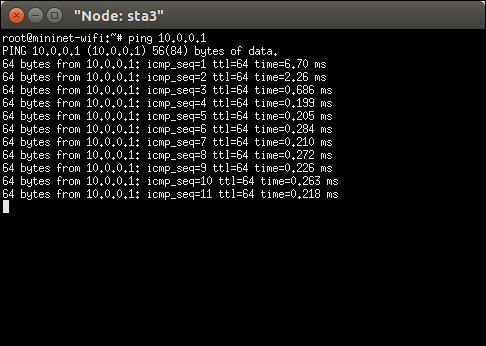
\includegraphics[width=0.7\textwidth]{Pictures/mn-wifi-102.png}
    \caption{xterm window on sta3}
    \label{fig:xterm}
\end{figure}


In that window, run the following command to send ICMP messages from \texttt{sta3} to \texttt{sta1}:     

\begin{minted}{bash}
    root@mininet-wifi:~# ping 10.0.0.1
\end{minted}

Since these packets will be forwarded by the associated access points out a port other then the port on which the packets were received, the access points will operate like normal OpenFlow-enabled switches. Each access point will forward the first ping packet it receives in each direction to the Mininet reference controller. The controller will set up flows on the access points to establish a connection between the stations \texttt{sta1} and \texttt{sta3}.

If we run Wireshark (figure~\ref{fig:wireshark} and enable packet capture on the \texttt{Loopback} interface, then filter using with \texttt{of} (for Ubuntu 14.04) or \texttt{openflow\_v1} (for Ubuntu 15.10 and later), we will see OpenFlow messages passing to and from the controller. Now, in the Mininet CLI, check the flows on each switch with the \texttt{dpctl dump-flows} command.

\begin{figure}
    \centering
    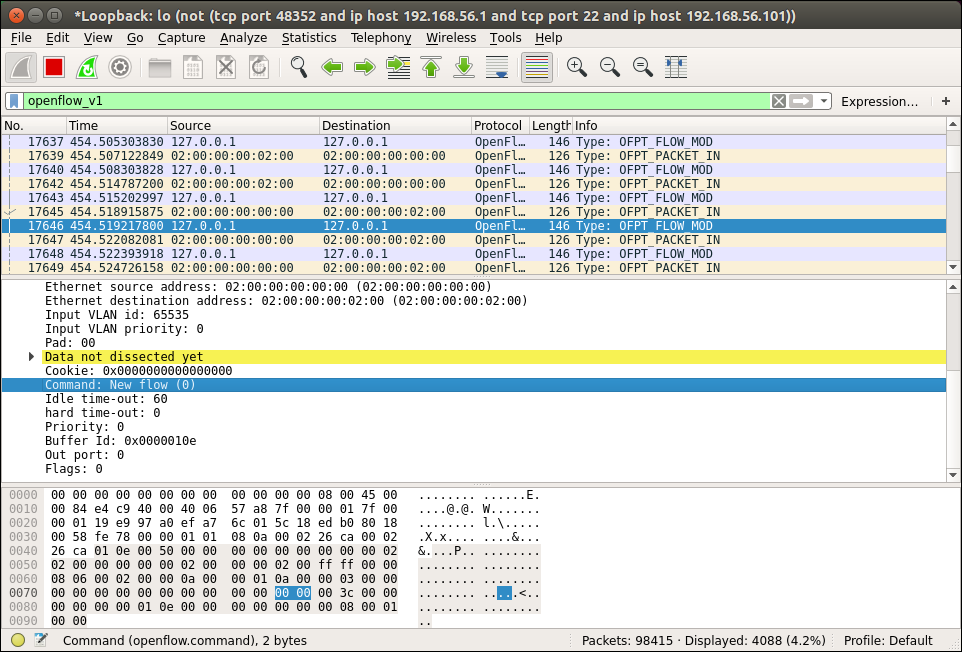
\includegraphics[width=0.8\textwidth]{Pictures/mn-wifi-121.png}
    \caption{Wireshark capturing OpenFlow messages}
    \label{fig:wireshark}
\end{figure}

\begin{minted}[breaklines]{bash}
mininet-wifi> dpctl dump-flows
    *** ap1 -----------------------------------------------
    NXST_FLOW reply (xid=0x4):
    *** ap2 -----------------------------------------------
    NXST_FLOW reply (xid=0x4):
    idle_timeout=60, idle_age=0, priority=65535,arp,in_port=2,vlan_tci=0x0000,dl_src=02:00:00:00:02:00, dl_dst=02:00:00:00:00:00,arp_spa=10.0.0.3,arp_tpa=10.0.0.1,arp_op=2 actions=output:3
     cookie=0x0, duration=1068.17s, table=0, n_packets=35, n_bytes=1470, idle_timeout=60, idle_age=0, priority=65535,arp,in_port=3,vlan_tci=0x0000,dl_src=02:00:00:00:00:00, dl_dst=02:00:00:00:02:00,arp_spa=10.0.0.1,arp_tpa=10.0.0.3,arp_op=1 actions=output:2
     cookie=0x0, duration=1073.174s, table=0, n_packets=1073, n_bytes=105154, idle_timeout=60, idle_age=0, priority=65535,icmp,in_port=3,vlan_tci=0x0000,dl_src=02:00:00:00:00:00, dl_dst=02:00:00:00:02:00,nw_src=10.0.0.1,nw_dst=10.0.0.3,nw_tos=0, icmp_type=0,icmp_code=0 actions=output:2
     cookie=0x0, duration=1073.175s, table=0, n_packets=1073, n_bytes=105154, idle_timeout=60, idle_age=0, priority=65535,icmp,in_port=2,vlan_tci=0x0000,dl_src=02:00:00:00:02:00, dl_dst=02:00:00:00:00:00,nw_src=10.0.0.3,nw_dst=10.0.0.1,nw_tos=0, icmp_type=8,icmp_code=0 actions=output:3
    *** ap3 -----------------------------------------------
    NXST_FLOW reply (xid=0x4):
     cookie=0x0, duration=1068.176s, table=0, n_packets=35, n_bytes=1470, idle_timeout=60, idle_age=0, priority=65535,arp,in_port=2,vlan_tci=0x0000,dl_src=02:00:00:00:02:00, dl_dst=02:00:00:00:00:00,arp_spa=10.0.0.3,arp_tpa=10.0.0.1,arp_op=2 actions=output:1
    idle_timeout=60, idle_age=0, priority=65535,arp,in_port=1,vlan_tci=0x0000,dl_src=02:00:00:00:00:00, dl_dst=02:00:00:00:02:00,arp_spa=10.0.0.1,arp_tpa=10.0.0.3,arp_op=1 actions=output:2
     cookie=0x0, duration=1073.182s, table=0, n_packets=1073, n_bytes=105154, idle_timeout=60, idle_age=0, priority=65535,icmp,in_port=1,vlan_tci=0x0000,dl_src=02:00:00:00:00:00, dl_dst=02:00:00:00:02:00,nw_src=10.0.0.1,nw_dst=10.0.0.3,nw_tos=0, icmp_type=0,icmp_code=0 actions=output:2
     cookie=0x0, duration=1073.185s, table=0, n_packets=1073, n_bytes=105154, idle_timeout=60, idle_age=0, priority=65535,icmp,in_port=2,vlan_tci=0x0000,dl_src=02:00:00:00:02:00, dl_dst=02:00:00:00:00:00,nw_src=10.0.0.3,nw_dst=10.0.0.1,nw_tos=0, icmp_type=8,icmp_code=0 actions=output:1
mininet-wifi>
\end{minted} 

We see flows set up on \texttt{ap2} and \texttt{ap3}, but not on \texttt{ap1}. This is because \texttt{sta1} is connected to \texttt{ap2} and \texttt{sta3} is connected to \texttt{ap3} so all traffic is passing through only \texttt{ap2} and \texttt{ap3}. What will happen if \texttt{sta1} moves back to \texttt{ap1}? Move \texttt{sta1} back to access point \texttt{ap1} with the following commands:

\begin{minted}{bash}
    mininet-wifi> sta1 iw dev sta1-wlan0 disconnect
    mininet-wifi> sta1 iw dev sta1-wlan0 connect ssid_ap1
\end{minted}

The \texttt{ping} command running on \texttt{sta3} stops working. We see no more pings completed.

In this case, access points \texttt{ap2} and \texttt{ap3} already have flows for ICMP messages coming from \texttt{sta3} so they just keep sending packets towards the \texttt{ap2-wlan0} interface to reach where they think \texttt{sta1} is connected. Since ping messages never get to \texttt{sta1} in its new location, the access point \texttt{ap1} never sees any ICMP traffic so does not request any flow updates from the controller.

Check the flow tables in the access points again: 

\begin{minted}[breaklines]{bash}
mininet-wifi> dpctl dump-flows
    *** ap1 -----------------------------------------------
    NXST_FLOW reply (xid=0x4):
     cookie=0x0, duration=40.959s, table=0, n_packets=1, n_bytes=42, idle_timeout=60, idle_age=40, priority=65535,arp,in_port=1,vlan_tci=0x0000,dl_src=02:00:00:00:02:00, dl_dst=02:00:00:00:00:00,arp_spa=10.0.0.3,arp_tpa=10.0.0.1,arp_op=1 actions=output:2
     cookie=0x0, duration=40.958s, table=0, n_packets=1, n_bytes=42, idle_timeout=60, idle_age=40, priority=65535,arp,in_port=2,vlan_tci=0x0000,dl_src=02:00:00:00:00:00, dl_dst=02:00:00:00:02:00,arp_spa=10.0.0.1,arp_tpa=10.0.0.3,arp_op=2 actions=output:1
    *** ap2 -----------------------------------------------
    NXST_FLOW reply (xid=0x4):
     cookie=0x0, duration=40.968s, table=0, n_packets=1, n_bytes=42, idle_timeout=60, idle_age=40, priority=65535,arp,in_port=2,vlan_tci=0x0000,dl_src=02:00:00:00:02:00, dl_dst=02:00:00:00:00:00,arp_spa=10.0.0.3,arp_tpa=10.0.0.1,arp_op=1 actions=output:1
     cookie=0x0, duration=40.964s, table=0, n_packets=1, n_bytes=42, idle_timeout=60, idle_age=40, priority=65535,arp,in_port=1,vlan_tci=0x0000,dl_src=02:00:00:00:00:00, dl_dst=02:00:00:00:02:00,arp_spa=10.0.0.1,arp_tpa=10.0.0.3,arp_op=2 actions=output:2
     cookie=0x0, duration=1214.279s, table=0, n_packets=1214, n_bytes=118972, idle_timeout=60, idle_age=0, priority=65535,icmp,in_port=2,vlan_tci=0x0000,dl_src=02:00:00:00:02:00, dl_dst=02:00:00:00:00:00,nw_src=10.0.0.3,nw_dst=10.0.0.1,nw_tos=0, icmp_type=8,icmp_code=0 actions=output:3
    *** ap3 -----------------------------------------------
    NXST_FLOW reply (xid=0x4):
     cookie=0x0, duration=40.978s, table=0, n_packets=1, n_bytes=42, idle_timeout=60, idle_age=40, priority=65535,arp,in_port=2,vlan_tci=0x0000,dl_src=02:00:00:00:02:00, dl_dst=02:00:00:00:00:00,arp_spa=10.0.0.3,arp_tpa=10.0.0.1,arp_op=1 actions=output:1
     cookie=0x0, duration=40.971s, table=0, n_packets=1, n_bytes=42, idle_timeout=60, idle_age=40, priority=65535,arp,in_port=1,vlan_tci=0x0000,dl_src=02:00:00:00:00:00, dl_dst=02:00:00:00:02:00,arp_spa=10.0.0.1,arp_tpa=10.0.0.3,arp_op=2 actions=output:2
     cookie=0x0, duration=1214.288s, table=0, n_packets=1214, n_bytes=118972, idle_timeout=60, idle_age=0, priority=65535,icmp,in_port=2,vlan_tci=0x0000,dl_src=02:00:00:00:02:00, dl_dst=02:00:00:00:00:00,nw_src=10.0.0.3,nw_dst=10.0.0.1,nw_tos=0, icmp_type=8,icmp_code=0 actions=output:1
mininet-wifi>
\end{minted}    

The controller sees some LLC messages from \texttt{sta1} but does recognize that \texttt{sta1} has moved to a new access point, so it does nothing. Since the controller does not modify any flows in the access points, none of the ICMP packets still being generated by \texttt{sta3} will reach \texttt{sta1} so it cannot reply. This situation will remain as long as the access points \texttt{ap2} and \texttt{ap3} continue to see ICMP packets from \texttt{sta3}, which keeps the old flow information alive in their flow tables.

One "brute force" way to resolve this situation is to delete the flows on the switches. In this simple example, it's easier to just delete all flows. Delete the flows in the access points using the command below: 

\begin{minted}{bash}
    mininet-wifi> dpctl del-flows
\end{minted}
    

Now the ping command running in the xterm window on \texttt{sta3} should show that pings are being completed again.

Once all flows were deleted, ICMP messages received by the access points do not match any existing flows so the access points communicate with the controller to set up new flows. If we dump the flows we see that the ICMP packets passing between \texttt{sta3} and \texttt{sta1} are now traversing across all three acces points.

\begin{minted}[breaklines]{bash}
mininet-wifi> dpctl dump-flows
    *** ap1 -----------------------------------------------
    NXST_FLOW reply (xid=0x4):
     cookie=0x0, duration=10.41s, table=0, n_packets=11, n_bytes=1078, idle_timeout=60, idle_age=0, priority=65535,icmp,in_port=2,vlan_tci=0x0000,dl_src=02:00:00:00:00:00, dl_dst=02:00:00:00:02:00,nw_src=10.0.0.1,nw_dst=10.0.0.3,nw_tos=0, icmp_type=0,icmp_code=0 actions=output:1
     cookie=0x0, duration=9.41s, table=0, n_packets=10, n_bytes=980, idle_timeout=60, idle_age=0, priority=65535,icmp,in_port=1,vlan_tci=0x0000,dl_src=02:00:00:00:02:00, dl_dst=02:00:00:00:00:00,nw_src=10.0.0.3,nw_dst=10.0.0.1,nw_tos=0, icmp_type=8,icmp_code=0 actions=output:2
    *** ap2 -----------------------------------------------
    NXST_FLOW reply (xid=0x4):
     cookie=0x0, duration=10.414s, table=0, n_packets=11, n_bytes=1078, idle_timeout=60, idle_age=0, priority=65535,icmp,in_port=1,vlan_tci=0x0000,dl_src=02:00:00:00:00:00, dl_dst=02:00:00:00:02:00,nw_src=10.0.0.1,nw_dst=10.0.0.3,nw_tos=0, icmp_type=0,icmp_code=0 actions=output:2
     cookie=0x0, duration=9.417s, table=0, n_packets=10, n_bytes=980, idle_timeout=60, idle_age=0, priority=65535,icmp,in_port=2,vlan_tci=0x0000,dl_src=02:00:00:00:02:00, dl_dst=02:00:00:00:00:00,nw_src=10.0.0.3,nw_dst=10.0.0.1,nw_tos=0, icmp_type=8,icmp_code=0 actions=output:1
    *** ap3 -----------------------------------------------
    NXST_FLOW reply (xid=0x4):
     cookie=0x0, duration=10.421s, table=0, n_packets=11, n_bytes=1078, idle_timeout=60, idle_age=0, priority=65535,icmp,in_port=1,vlan_tci=0x0000,dl_src=02:00:00:00:00:00, dl_dst=02:00:00:00:02:00,nw_src=10.0.0.1,nw_dst=10.0.0.3,nw_tos=0, icmp_type=0,icmp_code=0 actions=output:2
     cookie=0x0, duration=9.427s, table=0, n_packets=10, n_bytes=980, idle_timeout=60, idl_age=0, priority=65535,icmp,in_port=2,vlan_tci=0x0000,dl_src=02:00:00:00:02:00, dl_dst=02:00:00:00:00:00,nw_src=10.0.0.3,nw_dst=10.0.0.1,nw_tos=0, icmp_type=8,icmp_code=0 actions=output:1
mininet-wifi>
\end{minted}
    

We have shown how the Mininet reference controller works in Mininet-WiFi. The Mininet reference controller does not have the ability to detect when a station moves from one access point to another. When this happens, we must delete the existing flows so that new flows can be created. We will need to us a more advanced remote controller, such as OpenDaylight, to enable station mobility but that is a topic outside the scope of this post.

\subsection{Stop the tutorial}

Stop the Mininet \texttt{ping} command by pressing \texttt{Ctrl-C}. In the Wireshark window, stop capturing and quit Wireshark. Stop Mininet-Wifi and clean up the system with the following commands:

\begin{minted}{bash}
    mininet-wifi> exit
    wifi:~$ sudo mn -c
\end{minted}

\section{Mininet-WiFi Tutorial \#3: Python API and scripts}

Mininet provides a Python API so users can create simple Python scripts that will set up custom topologies. Mininet-WiFi extends this API to support a wireless environment.

When you use the normal Mininet \texttt{mn} command with the \texttt{--wifi} option to create Mininet-WiFi topologies, you do not have access to most of the extended functionality provided in Mininet-WiFi. To access features that allow you to emulate the behavior of nodes in a wireless LAN, you need to use the Mininet-Wifi extensions to the Mininet Python API.

\subsection{The Mininet-WiFi Python API}

The Mininet-WiFi developers added new classes to Mininet to support emulation of nodes in a wireless environment. Mininet-WiFi adds \texttt{addStation} and \texttt{addAccessPoint} methods, and a modified \texttt{addLink} method to define the wireless environment. 

If you are just beginning to write scripts for Mininet-WiFi, you can use the example scripts as a starting point. The Mininet-WiFi developers created example scripts that show how to use most of the features in Mininet-WiFi. In all of the tutorials I show below, I started with an example script and modified it. 

Mininet-Wifi example scripts are in the \texttt{~/mininet-wifi/examples} directory.

\subsection{Basic station and access point methods}

In a simple scenario, you may add a station and an access point with the following methods in a Mininet-WiFi Python script: \\

\noindent Add a new station named \texttt{sta1}, with all parameters set to default values:

\begin{minted}{bash}
    net.addStation( 'sta1' )
\end{minted}
    

\noindent Add a new access point named \texttt{ap1}, with SSID \texttt{ap1-ssid}, and all other parameters set to default values:
    
\begin{minted}{bash}
    net.addAccessPoint( 'ap1',  ssid='new_ssid' )
\end{minted}

\noindent Add a wireless association between station and access point, with default values for link attributes:

\begin{minted}{bash}
    net.addLink( ap1, sta1 )
\end{minted}
    
\noindent For more complex scenarios, more parameters are available for each method. You may specify the MAC address, IP address, location in three dimensional space, radio range, and more. For example, the following code defines an access point and a station, and creates an association (a wireless connection) between the two nodes and applies some traffic control parameters to the connection to make it more like a realistic radio environment, adding badwidth restrictions, an error rate, and a propagation delay:\\

\noindent Add a station and specify the wireless encryption method, the station MAC address, IP address, and position in virtual space:

\begin{minted}[breaklines]{bash}
    net.addStation( 'sta1', passwd='123456789a', encrypt='wpa2', mac='00:00:00:00:00:02', ip='10.0.0.2/8', position='50,30,0' ) 
\end{minted}
       
\noindent Add an access point and specify the wireless encryption method, SSID, wireless mode, channel, position, and radio range:

\begin{minted}[breaklines]{bash}
    net.addAccessPoint( 'ap1', passwd='123456789a', encrypt='wpa2', ssid= 'ap1-ssid', mode= 'g', channel= '1', position='30,30,0', range=30 )
\end{minted}    

To activate association control in a static network, you may use the *associationControl* method, which makes Mininet-WiFi automatically choose which access point a station will connect to based on the range between stations and access points. For example, use the following method to use the *strongest signal first* when determining connections between station and access points:

\begin{minted}{bash}
    net.associationControl( 'ssf' )
\end{minted}
    
\subsection{Classic Mininet API}

The Mininet WiFi Python API still supports the standard Mininet node types -- switches, hosts, and controllers. For example:\\

\noindent Add a host. Note that the station discussed above is a type of host nodem with a wireless interface instead of an Ehternet interface.

\begin{minted}{bash}
    net.addHost( 'h1' )
\end{minted}
    

\noindent Add a switch. Note that the access point discussed above is a type of switch that has one wireless interface (*wlan0*) and any number of Ethernet interfaces (up to the maximum supported by your installed version of Open vSwitch).

\begin{minted}{bash}
    net.addSwitch( 's1' )
\end{minted}
    

\noindent Add an Ethernet link between two nodes. Note that if you use *addLink* to connect two access points together (and are using the default Infrastructure mode), Mininet-WiFi creates an Ethernet link between them.

\begin{minted}{bash}
    net.addLink( s1, h1 )
\end{minted}
    
\noindent Add a controller:

\begin{minted}{bash}
    net.addController( 'c0' )
\end{minted}
        
\noindent Using the Python API, you may build a topology that includes hosts, switches, stations, access points, and multiple controllers.

\subsection{ Example }

In the example below, I created a Python program that will set up two stations connected to two access points, and set node positions and radio range so that we can see how these properties affect the emulated network. I used the Mininet-WiFi example script \texttt{2AccessPoints.py} as the base for the script shown below, then I added the position information to each node and enabled association control.

\lstinputlisting[language=Python]{codes/position-test.py}

I saved the file with the name \texttt{position-test.py} and made it executable. 

\subsection{Working at runtime}

Mininet-WiFi python scripts may be run from the command line by running the script directly, or by calling it as part of a Python command. The only difference is how the path is stated. For example:

\begin{minted}{bash}
    wifi:~/scripts $ sudo ./position-test.py
\end{minted}
or,
\begin{minted}{bash}
    wifi:~$ sudo python position-test.py
\end{minted}

The \texttt{position-test.py} script will set open the Mininet-WiFi graph window and show the locations of each wireless node in space (figure~\ref{fig:scriptrunning}, and the range attribute of each node.

\begin{figure}
    \centering
    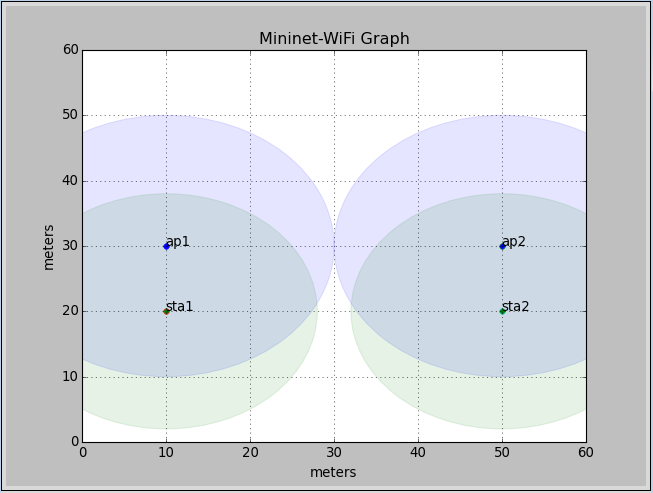
\includegraphics[width=0.7\textwidth]{Pictures/mn-wifi-graph-300.png}
    \caption{The position-test.py script running}
    \label{fig:scriptrunning}
\end{figure}

While the scenario is running, we can query information about the network from either the Mininet-WiFi command line or from the Python interpreter and we can log into running nodes to gather information or make configuration changes.

\subsection{Mininet-WiFi CLI}

The Python script \texttt{position-test.py} places nodes in specific positions. When the scenario is running, we can use the Mininet-WiFi command line interface (CLI) commands to can check the geometric relationship between nodes in space, and information about each node.

\subsection{Position}

The \texttt{position} CLI command outputs the location of a node in virtual space as measured by three values, one for each of the vertices X, Y, and Z.

Suppose we want to know the position of the access point \texttt{ap1} in the network scenario's virtual space. We may use the \texttt{position} CLI command to view a node's position:

\begin{minted}{bash}
    mininet-wifi> py ap1.params['position']
\end{minted}
   

We may also check the position of the station \texttt{sta2}:

\begin{minted}{bash}
    mininet-wifi> py sta.params['position']
\end{minted}
  
\subsection{Distance}

The \texttt{distance} CLI command tells us the distance between two nodes. For example, we may check how far apart access point \texttt{ap1} and station \texttt{sta2} are from each other using the \texttt{distance} CLI command:

\begin{minted}{bash}
    mininet-wifi> distance ap1 sta2        
    The distance between ap1 and sta2 is 41.23 meters
\end{minted}
       
\subsection{Mininet-WiFi Python runtime interpreter}

In addition to the CLI, Mininet-WiFi supports running Python code directly at the command line using the \texttt{py} command. Simple, Python functions may be called to get additional information about the network, or to make simple changes while the scenario is running.

\subsection{Getting network information}

The examples I show below are useful for gathering information about stations and access points.

To see the range of an access point or station, call the \texttt{range} function. Call it using the name of the node followed by the function as shown below for access point \texttt{ap1}:

\begin{minted}{bash}
    mininet-wifi> py ap1.params['range']
    20
\end{minted}
    
\noindent To see which station is associated with an access point (in this example \texttt{ap1}) call the \texttt{associatedStations} function:

\begin{minted}{bash}
    mininet-wifi> py ap1.associatedStations
    [<Host sta1: sta1-wlan0:10.0.0.1 pid=3845> ]
\end{minted}
   
\noindent To see which access point is associated with a station (in this example \texttt{sta1}) call the \texttt{associatedTo} key:

\begin{minted}{bash}
    mininet-wifi>py sta1.params['associatedTo']
    [<OVSSwitch ap1: lo:127.0.0.1,ap1-eth1:None pid=3862>]
\end{minted}
        

\noindent You may also query the received signal strength indicator (\texttt{rssi}), transmitted power (\texttt{txpower}), service set indicator (\texttt{ssid}), \texttt{channel}, and \texttt{frequency} of each wireless node using the Python interpreter.

\noindent As we can see, the output of Python functions is formatted as strings and numbers that may sometimes be hard to read. This is because these functions are built to support the program, not to be read by humans. However, if you which functions are available to be called at the Mininet-WiFi command line you will be able to get information you cannot get through the standard Mininet-WiFi CLI.

\subsection{Changing the network during runtime}

Mininet-WiFi provides Python functions that can be used during runtime to make changes to node positions and associations. These functions are useful when we have a static setup and want to make arbitrary changes on demand. This makes it possible to do testing or demonstrations with carefully controlled scenarios.

To change the access point to which a station is associated (provided the access point is within range):

\begin{minted}{bash}
    sta1.moveAssociationTo('sta1-wlan0', 'ap1') 
\end{minted}
    

\noindent To move a station or access point in space to another coordinate position:

\begin{minted}{bash}
    sta1.moveNodeTo('40,20,40')
\end{minted}
    
\noindent To change the range of a station or access point:

\begin{minted}{bash}
    sta1.setRange(100)
\end{minted}    

The commands above will all impact which access points and which stations associate with each other. The behavior of the network will be different depending on whether association control is enabled or disabled in the \texttt{position-test.py} script.

\subsection{Running commands in nodes}

When running a scenario, users may make configuration changes on nodes to implement some additional functionality. This can be done from the Mininet-WiFi command line by sending commands to the node's command shell. Start the command with the name of the node followed by a space, then enter the command to run on that node.

\noindent For example, to see information about the WLAN interface on a station named \texttt{sta1}, run the command:

\begin{minted}{bash}
    mininet-wifi> sta1 iw dev sta1-wlan0 link
\end{minted}
    

\noindent Another way to run commands on nodes is to open an \texttt{xterm} window on that node and enter commands in the xterm window. For example, to open an xterm window on station *sta1*, run the command:

\begin{minted}{bash}
    mininet-wifi> xterm sta1
\end{minted}
    

\noindent Running commands on nodes is standard Mininet feature but it is also an advanced topic. See the \texttt{Mininet documentation}\footnote{https://github.com/mininet/mininet/wiki/Documentation} for more details. You can run simple commands such as \texttt{ping} or \texttt{iwconfig} but more advance commands may require you to mount \texttt{private directories}\footnote{https://github.com/mininet/mininet/wiki/Introduction-to-Mininet\#important-shared-filesystem} for configuration or log files.

\subsection{Mininet-WiFi and shell commands}

Mininet-WiFi manages the affect of range using code that calculates the ability of each node to connect with other nodes. However, Mininet-WiFi does not change the way networking works at the operating system level. So \texttt{iw} commands executed on nodes will override Mininet-WiFi and do not gather information generated by Mininet-WiFi about the network.

I suggest you do not rely on \texttt{iw} commands. For example, the \texttt{iw scan} command will still show that \texttt{sta1} can detect the SSIDs of all access points, even the access point \texttt{ap2} which should be out of range. The \texttt{iw link} command will show the same signal strength regardless of how far the station is from the access point, while the Mininet-WiFi *info* command will show the calculated signal strength based on the propagation model and distance between nodes.

For example, the \texttt{iw} command run on \texttt{sta1} shows received signal strength is -30 dBm. This never changes no matter how far the station is from the access point.


\begin{minted}{bash}
mininet-wifi> sta1 iw dev sta1-wlan0 link
Connected to 02:00:00:00:00:00 (on sta1-wlan0)
        SSID: ssid-ap1
        freq: 2412
        RX: 164628 bytes (2993 packets)
        TX: 775 bytes (10 packets)
        signal: -30 dBm
        tx bitrate: 6.0 MBit/s

        bss flags:      short-slot-time
        dtim period:    2
        beacon int:     100
\end{minted}
    

The \texttt{info} command shows Mininet-WiFi's calculated signal strength received by the station is -43.11 dBm. This value will change if you reposition the station.


\subsection{Stop the tutorial}

Stop Mininet-Wifi and clean up the system with the following commands:


\begin{minted}{bash}
    mininet-wifi> exit
    wifi:~$ sudo mn -c
\end{minted}

\section{Mininet-WiFi Tutorial \#4: Mobility}

The more interesting features provided by Mininet-WiFi support mobile stations moving around in virtual space. Mininet-Wifi provides new methods in its Python API, such as \texttt{startMobility} and \texttt{Mobility}, with which we may specify a wide variety of wireless LAN scenarios by controlling station movement, access point range, radio propagation models, and more.

In this tutorial, we will create a scenario where one station moves about in space, and where it changes which access point it connects to, based on which access point is the closest.

\subsection{Python API and mobility}

The Mininet-WiFi Python API adds new methods that allow the user to create stations that move around in virtual space when an emulation scenario is running.

To move a station in a straight line, use the \texttt{net.StartMobility} and \texttt{net.mobility} methods. See the example script \texttt{wifiMobilty.py}. For example, to move a station from one position to another over a period of 60 seconds, add the following lines to your script:

\begin{minted}{bash}
    net.startMobility( time=0 )
    net.mobility( 'sta1', 'start', time=1, position='10,20,0' )
    net.mobility( 'sta1', 'stop', time=59, position='30,50,0' )
    net.stopMobility( time=60 )
\end{minted}

    

Mininet-WiFi can also automatically move stations around based on predefined mobility models. See the example script \texttt{wifiMobilityModel.py}. Available mobility models are: \texttt{RandomWalk}, \texttt{TruncatedLevyWalk}, \texttt{RandomDirection}, \texttt{RandomWayPoint}, \texttt{GaussMarkov}, \texttt{ReferencePoint}, and \texttt{TimeVariantCommunity}. For example, to move a station around in an area 60 meters by 60 meters with a minimum velocity of 0.1 meters per second and a maximum velocity of 0.2 meters per second, add the following line to your script:

\begin{minted}[breaklines]{bash}
    net.startMobility(time=0, model='RandomDirection', max_x=60, max_y=60, min_v=0.1, max_v=0.2)
\end{minted}    

Mininet-WiFi will automatically connect and disconnect stations to and from access points based on either calculated signal strength or load level. See the example script \texttt{wifiAssociationControl.py}. To use association control, add the \texttt{AC} parameter to the \texttt{net.startMobility} call. For example, to switch access points based on the “least loaded first” criteria, add the following line to your script:

\begin{minted}[breaklines]{bash}
    net.startMobility(time=0, model='RandomWayPoint', max_x=140, max_y=140, min_v=0.7, max_v=0.9, AC='llf')
\end{minted}

The valid values for the \texttt{AC} parameter are:

\begin{itemize}
\item llf (Least-Loaded-First)
\item ssf (Strongest-Signal-First)\\
\end{itemize}

When creating a scenario where stations will be mobile, we may set the range of the access points. In an example where we use “strongest signal first” as the Association Control method, the range of each access point will determine where handoffs occur between access points and which stations may connect to which access points. If you do not define the range, Mininet-WiFi assigns a default value. 

Mininet-WiFi supports more methods than mentioned above. See the example scripts (mentioned further below) for examples of using other methods.


\subsection{Moving a station in virtual space}

A simple way to demonstrate how Mininet-WiFi implements scenarios with mobile stations that hand off between access points is to create a script that moves one station across a path that passes by three access points.

The example below will create three access points -- \texttt{ap1}, \texttt{ap2}, and \texttt{ap3} -- arranged in a line at differing distances from each other. It also creates a host \texttt{h1} to serve as a test server and a mobile station \texttt{sta1} and moves \texttt{sta1} across space past all three access points.

\lstinputlisting[language=Python]{codes/line.py}

Save the script and call in \texttt{line.py}. Make it executable, then run the command:

\begin{minted}[breaklines]{bash}
    wifi:~$ sudo ./line.py
\end{minted} 

The Mininet-Wifi graph will appear (figure~\ref{fig:linescript}), showing the station and the access points. 

\begin{figure}[!b]
    \centering
    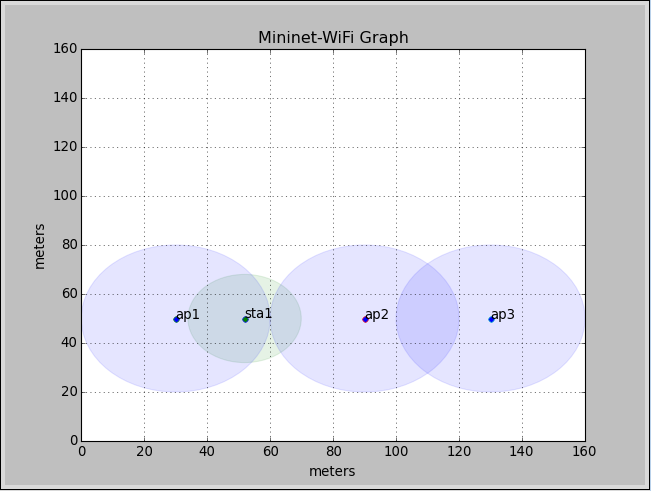
\includegraphics[width=0.7\textwidth]{Pictures/mn-wifi-graph-100}
    \caption{The line.py script running}
    \label{fig:linescript}
\end{figure}

The station \texttt{sta1} will sit still for 20 seconds, and then start to move across the graph from left to right for 60 seconds until it gets to the far side of the graph. The host \texttt{h1} and the virtual Ethernet connections between \texttt{h1}, \texttt{ap1} and between the three access points are not visible.

\subsection{Re-starting the scenario}

This simple scenario has a discreet start and stop time so, if you wish to run it again, you need to quit Mininet-WiFi, and start the script again. 

For example, suppose the scenario is at its end, where the station is now at the far right of the graph window. To stop and start it again, enter the following commands:

\begin{minted}{bash}
    mininet-wifi> exit
    wifi:~$ sudo mn -c
    wifi:~$ sudo ./line.py
\end{minted}    

\subsection{More Python functions}

When running a scenario with the mobility methods in the Python API, we have access to more information from Mininet-WiFi's Python functions. To see all access points that are within range of a station such as \texttt{sta1} at any time while the scenario is running, call the \texttt{apsInRange} function:

\begin{minted}{bash}
    mininet-wifi> py sta1.params['apsInRange']
    [<OVSSwitch ap1: lo:127.0.0.1,ap1-eth1:None pid=3862>]
\end{minted}
    
\subsection{Test with iperf}

To see how the system responds to traffic, run some data between host \texttt{h1} and station \texttt{sta1} when the scenario is started.\\

\noindent We have seen in previous examples how to use the \texttt{ping} program to create traffic. In this example, we will use the \texttt{iperf} program. First, start the \texttt{line.py} script again. Then start an iperf server on the station

\begin{minted}{bash}
    mininet-wifi> sta1 iperf --server 
\end{minted}
    

\noindent Then open an xterm window on the host \texttt{h1}. 

\begin{minted}{bash}
    mininet-wifi> xterm h1
\end{minted}
    

\noindent From the xterm window, we will start the iperf client command and create a stream of data between \texttt{h1} and \texttt{sta1}. On the \texttt{h1} xterm, run the command:

\begin{minted}{bash}
    iperf --client 10.0.0.2 --time 60 --interval 2 
\end{minted}

\noindent Watch the iperf output as the station moves through the graph. When it passes from one access point to the next, the traffic will stop. To get the traffic running again, clear the flow tables in the access points. In the Mininet-WiFi CLI, run the command shown below:

\begin{minted}{bash}
    mininet-wifi> dpctl del-flows
\end{minted}
    

\noindent Traffic should start running again. As stated in Tutorial \#2 above, we must clear flows after a hand off because the Mininet reference controller cannot respond correctly in a mobility scenario. The topic of configuring a remote controller to support a mobility scenario is outside the scope of this post. Clear the flows every time the station switches to the next access point.

\subsection{Stop the tutorial}

Stop Mininet-Wifi and clean up the system with the following commands:

\begin{minted}{bash}
    mininet-wifi> exit
    wifi:~$ sudo mn -c
\end{minted}

\section{Mininet-WiFi Tutorial \#5: VANETs (Veicular Ad Hoc Networks)}

\subsection{Python API}
The Mininet-WiFi python API add a new node that allow the user to create cars that move around in virtual space when an emulation scenario is running. The function addCar() defines this new node and you can see an example in the file vanet.py into /examples.

\subsection{Node Car Architecture}

The architecture of the node \texttt{car} is depicted in \autoref{fig:cararch}. In order to allow OpenFlow controllers to control simple nodes, like a car, it was necessary to create an architecture with a switch. Thus, every packet that comes from VehicleX needs to pass-trough VehicleXSW if the destination is a node in the wireless mesh network (like a Vehicle-to-Vehicle communication). The communication between cars and RSUs (Vehicle-to-Infrastructure), in turn, is done directly between VehicleX and the RSU. 

\begin{figure}[!t]
\centering
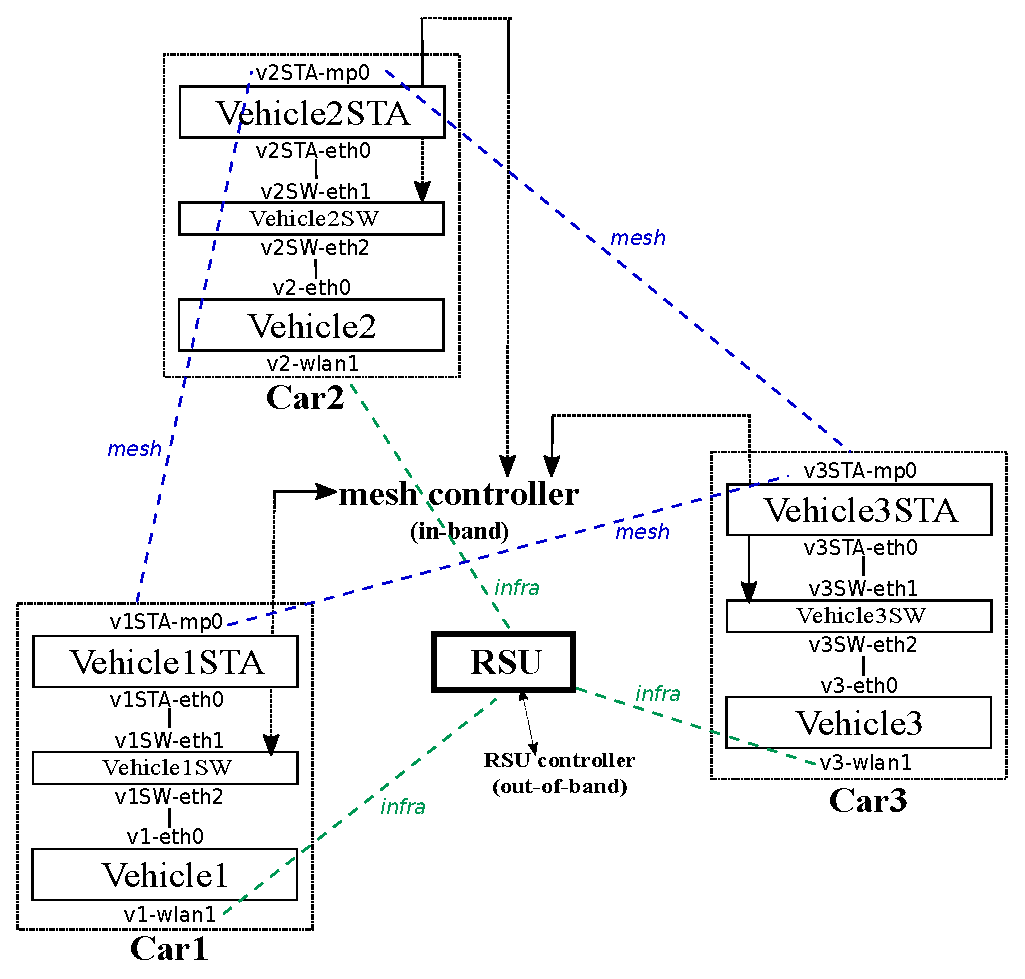
\includegraphics[width=0.6\textwidth]{Pictures/vanet.eps}
\caption{Node Car Architecture}
\label{fig:cararch}
\end{figure}

\begin{figure}[!b]
\centering
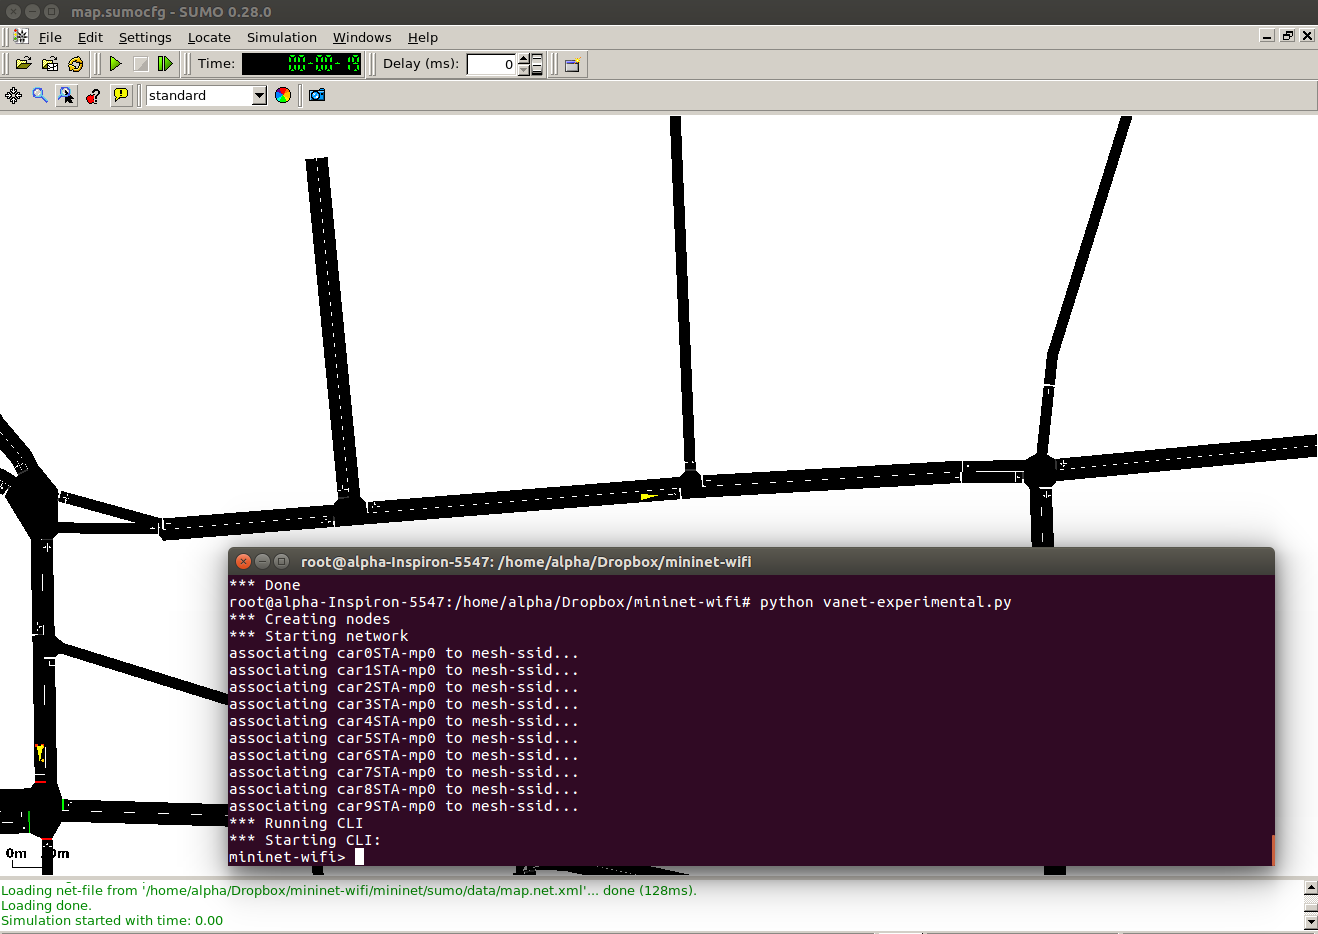
\includegraphics[width=0.6\textwidth]{Pictures/sumo.png}
\caption{Integration with SUMO}
\label{fig:sumo}
\end{figure}

\subsection{Integration with SUMO (Simulation of Urban Mobility)}
    
Mininet-WiFi already has some integration with SUMO. An example can be found in /examples/sumo-experimental.py.
    
\section{Mininet-WiFi example scripts}

The Mininet-WiFi developers created many example scripts that show examples of most of the API extensions they added to Mininet. They placed these example scripts in the folder \texttt{mininet-wifi/examples/}. Try running these scripts to see what they do and look at the code to understand how each feature is implemented using the Python API. Some interesting Mininet-WiFi example scripts are:

\texttt{adhoc} shows how to set up experiments with  adhoc mode, where stations connect to each other without passing through an access point.
\texttt{simplewifitopology} show the Python code that create the same topology as the default topology created my the \texttt{mn --wifi} command (two stations and one access point).
\texttt{wifiStationsAndHosts} creates a topology with stations and hosts
\texttt{2AccessPoints} to create a topology with two access points connected to each other via an Ethernet link and two stations associated with each access point.
\texttt{wifiPosition.py} shows how to create a network where stations and access points are places in specific locations in virtual space.
\texttt{wifiMobility} and \texttt{wifiMobilityModel} show how to move stations and how mobility models can be incorporated into scripts.
\texttt{wifiAssociationControl} shows how the different values of the AC parameter affect station handoffs to access points.
\texttt{wifimesh.py} shows how to set up a mesh network of stations.
\texttt{handover.py} shows how to create a simple mobility scenario where a station moves past two access points, causing the station to hand off from one to the other. 
\texttt{multipleWlan.py} shows how to create a station with more than one wireless LAN interface.
\texttt{wifiPropagationModel.py} shows how to use propagation models that impact how stations and access points can communicate with each other over distance.
\texttt{wifiAuthentication.py} shows how to set up WiFi encryption and passwords on access points and stations.

\section{Conclusion}

The tutorials presented above work demonstrate many of the unique functions offered by Mininet-Wifi. Each tutorial revealed more functionality and we stopped at the point where we were able to emulate mobility scenario featuring a WiFi station moving in a straight line past several wireless access points. 

To learn more about Mininet-WiFi, go to the \texttt{Mininet-WiFi wiki}\footnote{https://github.com/intrig-unicamp/mininet-wifi/wiki} page. Also, read through posts on the \texttt{Mininet-WiFi mailing list}\footnote{https://groups.google.com/forum/\#!forum/mininet-wifi-discuss}, which is very active and is a useful source of more information about Mininet-WiFi. I am looking for an OpenFlow controller that will support WiFi switches using OpenFlow 1.3, which is the version of OpenFlow supported by Mininet and Mininet-WiFi. If you know of any, please add a comment to this post.

\begin{remark}
Thank you Brian Linkletter for this helpful tutorial.
\end{remark}
\chapterimage{logo.png}
%%Chapter 1
%%%%%%%%%%%%%%%%%%%%%%%%%%%%%%%%%%%%%%%%%%%%%%%%%%%%%%%%%%%%%
\chapter{Guided exercises/demo}

\section{Guided exercises/demo}
In general, you will learn in this chapter how the Mininet-WiFi wireless network emulator works. Guided exercises will be explored and pointers to source code for those interested in delving deeper into the system architecture will be also provided. The pointers include stretches of the code where the link (including the latency) can be customized.


\subsection{Activity \themycounter{}: Warming up}   
\stepcounter{mycounter}

\noindent First of all, you have to stop the network-manager:

\begin{minted}{bash}
    sudo service network-manager stop 
\end{minted}


\noindent Then, create a simple topology with the command below:

\begin{minted}{bash}
    sudo mn --wifi
\end{minted}
	

\noindent The command above will start Mininet-WiFi and configure a small network with two stations, and one access point. Use the option {-}{-}topo of mn command, and discover further the topology options.

\noindent In Mininet-WiFi terminal (\textit{mininet-wifi>}), execute the command nodes to observe the created network. Then, execute iwconfig to verify the association between the stations and ap1.

\begin{minted}{bash}
    mininet-wifi>sta1 iwconfig
    mininet-wifi>sta2 iwconfig
    mininet-wifi>sta1 ping sta2
\end{minted}

	

\noindent Then, disconnect sta1 and confirm the disconnection:

\begin{minted}{bash}
    mininet-wifi>sta1 iw dev sta1-wlan0 disconnect
    mininet-wifi>sta1 iwconfig
    mininet-wifi>sta1 ping sta2
\end{minted}


\noindent Now, connect sta1 again: 

\begin{minted}{bash}
    mininet-wifi>sta1 iw dev sta1-wlan0 connect my-ssid
    mininet-wifi>sta1 iwconfig
    mininet-wifi>sta1 ping sta2
\end{minted}


\subsection{Activity \themycounter{}: Loading Network Topologies}

\noindent Running an example with the command below:
\begin{minted}{bash}
    sudo python examples/wifiPosition.py
\end{minted}


\noindent Now, observe the position of sta1, sta2 and ap1:
\begin{minted}{bash}
    mininet-wifi>py sta1.params['position']
    mininet-wifi>py sta2.params['position']
    mininet-wifi>py ap1.params['position']
\end{minted}



\noindent Observe the signal power as well:
\begin{minted}{bash}
    mininet-wifi>py sta1.params['rssi']
    mininet-wifi>py sta2.params['rssi']
\end{minted}


\noindent If you prefer, you can see the distance between two nodes with the following command:

\begin{minted}{bash}
    mininet-wifi>distance sta1 ap1
    mininet-wifi>distance sta1 sta2   
\end{minted}


\noindent \textbf{$\ast$ Question \themycounter.\thequestion{}\stepcounter{question}: What is the observed bandwidth between sta1 and sta2?}
\\\textit{\textbf{Tip}: try iperf sta1 sta2}
\\

\noindent Now, move sta1 to another position:
\begin{minted}{bash}
    mininet-wifi>py sta1.moveNodeTo('70,40,0')
\end{minted}


\noindent \textbf{$\ast$ Question \themycounter.\thequestion{}\stepcounter{question}: What happened with the association between sta1 and ap1?}
\\\textit{\textbf{Tip}: try sta1 iwconfig}
\\

\noindent Finally, increase the signal range of ap1:
\begin{minted}{bash}
    mininet-wifi>py ap1.setRange(60)
\end{minted}


\noindent \textbf{$\ast$ Question \themycounter.\thequestion{}\stepcounter{question}: What happened with the association between sta1 and ap1 now?}

\noindent \textbf{$\ast$ Question \themycounter.\thequestion{}\stepcounter{question}: Now, observe the bandwidth between sta1 and sta2 again. 
What can we conclude?  }


\stepcounter{mycounter}
\setcounter{question}{1}
\subsection{Activity \themycounter{}: Customizing the Wireless Channel}
	
Mininet-WiFi relies on the configuration of Linux TC (by default) to
control the wireless channel properties, such as \textit{bandwidth}, \textit{packet loss}, \textit{delay} and \textit{latency}. Please see the equations in \textit{mininet/wifiChannel.py} (refer to equationBW, equationLoss, equationDelay and equationLatency. Those equations can be customized by calling setChannelEquation(), for example:

\begin{minted}[breaklines]{bash}
    net.setChannelEquation(bw='value.rate * (1.1 ** -dist)', loss='(dist * 2)/100', delay='(dist / 10) + 1', latency='2 + dist')
\end{minted}

Alternatively, a new approach called wmediumd has been implemented, a wireless medium simulation tool for Linux, based on the netlink API implemented in the mac80211\_hwsim kernel driver. A couple of sample files that use wmediumd are available at /examples.\\

\noindent \textbf{$\ast$ Question \themycounter.\thequestion{}\stepcounter{question}: Run wifiPosition.py again and try \textit{sta1 tc qdisc} before and after moving sta1 to the new position. What do you can conclude about the configuration applied by tc?}
\\


%%Chapter 2
%%%%%%%%%%%%%%%%%%%%%%%%%%%%%%%%%%%%%%%%%%%%%%%%%%%%%%%%%%%%%
\section{Further hands-on}
(Further hands-on exercises proposed to be carried by the attendees on their own and at their pace.
	A number practical exercises will be proposed where mobility and/or distance (or poor signal) among mobile nodes may impact latency and bandwidth, consequently the communication between two nodes.)


\stepcounter{mycounter}
\setcounter{question}{1}
\subsection{Activity \themycounter{}: Mobility}  


\noindent Open examples/wifiMobilityModel.py with any text editor and change the velocity of stations as below:
\begin{minted}[breaklines]{bash}
   from: net.startMobility(time=0, model='RandomDirection', max_x=100, max_y=100, min_v=0.5, max_v=0.8)
   to: net.startMobility(time=0, model='RandomDirection', max_x=100, max_y=100, min_v=0.1, max_v=0.1)
\end{minted}

\noindent Run examples/wifiMobilityModel.py and change the signal range of ap1:
\begin{minted}{bash}
    python examples/wifiMobilityModel.py
    mininet-wifi>py ap1.setRange(60)
\end{minted}

\noindent Then, ping sta1 and sta2:
\begin{minted}{bash}
    mininet-wifi>sta1 ping sta2
\end{minted}

\noindent \textbf{$\ast$ Question \themycounter.\thequestion{}\stepcounter{question}: What can you conclude about the latency?}\\
\textit{\textbf{Tip:} you can issue sta1 tc qdisc, repeatedly, to see the values applied by tc.}


\stepcounter{mycounter}
\setcounter{question}{1}
\subsection{Activity \themycounter{}: Received Signal Strength} 

\noindent Open examples/wifiPosition.py with any text editor and add sta3 at position='10,10,10' and set max\_z=100 in order to plot a 3d graph. Then, run examples/wifiPosition.py.\\

\noindent \textbf{$\ast$ Question \themycounter.\thequestion{}\stepcounter{question}: What is the received signal strength indicator (RSSI) observed from sta3?}
\\
\\
\noindent \textbf{$\ast$ Question \themycounter.\thequestion{}\stepcounter{question}: What is the average ping response time between sta2 and sta1? And sta3 and sta1? \textit{Note: define the number of packets to 10 (ping -c10)}.}


%%Chapter 3
%%%%%%%%%%%%%%%%%%%%%%%%%%%%%%%%%%%%%%%%%%%%%%%%%%%%%%%%%%%%%
\section{OpenFlow}
You will learn with this activity some basic concepts of the OpenFlow protocol, such as idle/hard timeout and identify the impact of the mobility in the communication. 

\stepcounter{mycounter}
\setcounter{question}{1}
\subsection{Activity \themycounter{}: Mobility and OpenFlow}

\noindent First of all you have to get the code from \url{https://github.com/ramonfontes/reproducible-research/blob/master/mininet-wifi/ACROSS-Sweden-2017/handover.py} and then run it with the command below (the content of handover.py is also available in \autoref{code-handover}):

\begin{minted}{bash}
    sudo python handover.py
\end{minted}

\noindent Now, keep h1 pinging to sta1
\begin{minted}{bash}
    mininet-wifi>h1 ping sta1
\end{minted}

\noindent \textbf{$\ast$ Question \themycounter.\thequestion{}\stepcounter{question}: As you can see, h1 cannot reach sta1 when sta1 goes to ap2. Why? Two important commands should help you to answer this question:}

\begin{minted}{bash}
    mininet-wifi>links 
    mininet-wifi>sh ovs-ofctl dump-flows s3 
\end{minted}
\textit{\textbf{Tip:} Observe both idle\_timeout and idle\_age.}\\

\noindent \textbf{$\ast$ Question \themycounter.\thequestion{}\stepcounter{question}: Now you know the answer to Question 6.1, how could sta1 be reached by h1?}
\chapterimage{logo.png}
\chapter{Reproducible Research}

The code and instructions used in this section can be found at \url{https://github.com/ramonfontes/reproducible-research}

\section{SwitchOn 2015}
\textit{Extended abstract - Towards an Emulator for Software Defined Wireless Networks}\\
\textbf{}
\\
Firstly, you have to get the code at \url{https://github.com/ramonfontes/reproducible-research/blob/master/mininet-wifi/SWITCHON-2015}, then execute it:

\begin{minted}{bash}
sudo python allWirelessNetworksAroundUs.py
\end{minted}

\begin{minted}{bash}
mininet-wifi> xterm sta1 h1
\end{minted}

\noindent On sta1:
\begin{minted}[breaklines]{bash}
 cvlc -vvv v4l2:///dev/video0 --input-slave=alsa://hw:1,0 --mtu 1000 --sout'#transcode{vcodec=mp4v,vb=800,scale=1,acodec=mpga,ab=128,channels=1}: duplicate{dst=display,dst=rtp{sdp=rtsp://10.0.0.10:8080/helmet.sdp}'
\end{minted}

\noindent On h1:
\begin{minted}[breaklines]{bash}
cvlc rtsp://10.0.0.10:8080/helmet.sdp
\end{minted}

\section{SBRC 2016}
\textit{DEMO - Mininet-WiFi: Emulação de Redes Sem Fio Definidas por Software com suporte a Mobilidade}

Codes necessary to reproduce this paper are available at \url{https://github.com/ramonfontes/reproducible-research/tree/master/mininet-wifi/SBRC-2016}

\subsection{Case 1 - Simple test}
\begin{minted}[breaklines]{bash}
sudo mn --wifi  
mininet-wifi>sta1 ping sta2  
mininet-wifi>sta1 iwconfig  
mininet-wifi>sta2 iwconfig
\end{minted}
   
\subsection{Case 2 (1/2) - Communication among stations and hosts/Verifying flow table}
\begin{minted}[breaklines]{bash}
sudo python examples/wifiStationsAndHosts.py  
mininet-wifi>nodes  
mininet-wifi>sh ovs-ofctl dump-flows ap1  
mininet-wifi>sta1 ping h3  
mininet-wifi>sh ovs-ofctl dump-flows ap1 
\end{minted}

\subsection{Case 2 (2/2) - Changing the controller (from reference to external controller)}

Open the code examples/wifiStationsAndHosts.py and make the following changes:

\begin{minted}[breaklines]{bash}
from: net = Mininet( controller=Controller, link=TCLink, switch=OVSKernelSwitch )  
to: net = Mininet( controller=RemoteController, link=TCLink, switch=OVSKernelSwitch )  
from: c0 = net.addController('c0', controller=Controller, ip='127.0.0.1' )  
to: c0 = net.addController('c0', controller=RemoteController, ip='127.0.0.1' )  
sudo python examples/wifiStationsAndHosts.py  
mininet-wifi>sta1 ping h3  #Why there is no communication? 
\end{minted}
  
\subsection{Case 3 - Handover}
\begin{minted}[breaklines]{bash}
sudo python examples/handover.py  
mininet-wifi>sta1 iwconfig  
mininet-wifi>sta1 ping sta2  #here I suggest you wait sta1 reaches ap2 before going to the next step
mininet-wifi>sta1 iwconfig  
\end{minted}
 
\subsection{Case 4 - Changes at runtime}
\begin{minted}[breaklines]{bash}
sudo python examples/wifiPosition.py  
mininet-wifi>sta1 iwconfig   
mininet-wifi>sta1 ping sta2  
mininet-wifi>py sta1.moveNodeTo('70,40,0')  
mininet-wifi>sta1 iwconfig  
mininet-wifi>sta1 ping sta2  
mininet-wifi>py ap1.setRange(60)  
mininet-wifi>sta1 iwconfig  
mininet-wifi>sta1 ping sta2  
\end{minted}

\subsection{Case 5 - Bridging physical and virtual emulated environments}

\begin{minted}[breaklines]{bash}
sudo systemctl stop network-manager
\end{minted}

Edit sbrc.py:

\begin{minted}[breaklines]{bash}
from: phyap1 = net.addPhysicalBaseStation( 'phyap1', ssid= 'SBRC16-MininetWiFi', mode= 'g', channel= '1', position='50,115,0', wlan='wlan11' )  
to: wlan11 to your usb wlan interface.
\end{minted}

Then,

\begin{minted}[breaklines]{bash}
sudo python sbrc.py
\end{minted}

At this moment users attending the conference will be invited to connect their mobile devices into the physical/emulated environment.

\section{SIGCOMM 2016}{\label{sec:sigcomm2016}}
\textit{Demo: Mininet-WiFi: A Platform for Hybrid Physical-Virtual Software-Defined Wireless Networking Research}

Requirements to reproduce:
\begin{itemize}
\item WiFi interface + (other WiFi or ethernet interface)
\item Floodlight OpenFlow controller
\item ofsoftswitch13 (you may install it with \textit{util/install.sh -3f}) - https://github.com/CPqD/ofsoftswitch13
\item Speedtest-cli
\item Codes are available at \url{https://github.com/ramonfontes/reproducible-research/tree/master/mininet-wifi/SIGCOMM-2016}
\end{itemize}

Important (changes in code - You have to set both Internet and wlan interfaces):
\begin{minted}[breaklines]{bash}
internetIface = 'eth0' # wired/wireless card.
usbDongleIface = 'wlan0' # wifi interface.
\end{minted}

\noindent Next, executing the Floodlight OpenFlow controller: 
\begin{minted}[breaklines]{bash}
sudo java -jar target/floodlight.jar
\end{minted}

\noindent Then,
\begin{minted}[breaklines]{bash}
   sudo py hybridVirtualPhysical.py
   mininet-wifi> sh ./rule.hybridVirtualPhysical
\end{minted}

Despite the content of \textit{rule.hybridVirtualPhysical} is included in \textit{hybridVirtualPhysical.py}, we have faced some troubles in floodlight controller. Thus, probably you have to execute rule.hybridVirtualPhysical after executing hybridVirtualPhysical.py.

Now, stations should be able to communicate with each other and with the Internet. You may use any station connected to any Access Point and try it out:
\begin{minted}[breaklines]{bash}
   mininet-wifi>xterm $station 
   $station>speedtest-cli
\end{minted}
Using speedtest-cli you can test both Download and Upload speed of your Internet connection. The available bandwidth is controlled by OpenFlow meter entries.\\

\noindent There is a web server accessible at 10.0.0.111 and according rules applied in rule.hybridVirtualPhysical, if you access 10.0.0.109 the traffic will be redirect to 10.0.0.111.\\
\\
\\
\textbf{Useful commands:}
\begin{minted}[breaklines]{bash}
sta1 iw dev sta1-wlan0 mpath dump #verify mesh routing information
sh dpctl unix:/tmp/ap3 stats-flow
sh dpctl unix:/tmp/ap3 stats-meter
sh dpctl unix:/tmp/ap3 meter-config
\end{minted}

\section{From Theory to Experimental Evaluation: Resource Management in Software-Defined Vehicular Networks}

Firstly, you have to get vanet.py at \url{https://github.com/ramonfontes/reproducible-research/blob/master/mininet-wifi/IEEE-Access-2017/vanet.py}

\begin{minted}[breaklines]{bash}
   sudo python vanet.py
\end{minted}

\noindent Please consider to watch: https://www.youtube.com/watch?v=kO3O9EwrP\_s

\section{The Computer Journal - How far can we go? Towards
Realistic Software-Defined Wireless
Networking Experiments}

Codes necessary to reproduce this paper are available at \url{https://github.com/ramonfontes/reproducible-research/tree/master/mininet-wifi/The-Computer-Journal-2017}

\subsection{\textit{Wireless n-Casting}}
\textbf{Requirements:\\}
\texttt{Floodlight} controller.
\\
\\
In order to reproduce this case, please follow the instructions below:
\\
\\
First, run the controller:
\begin{minted}[breaklines]{bash}
sudo java -jar target/floodlight.jar
\end{minted}


\noindent start the topology:
\begin{minted}[breaklines]{bash}
sudo python ncasting.py
\end{minted}

\noindent and finally install the rules:
\begin{minted}[breaklines]{bash}
sudo python ncasting-controller.py
\end{minted}

\subsection{\textit{Multipath TCP}}
\textbf{Requirements:\\}
You have to install \texttt{mptcp} and \texttt{ifstat} to reproduce this use case. \\
\\
In order to allow the communication we use pox controller with spanning tree enabled. This command can be used to enable spanning tree:
\begin{minted}[breaklines]{bash}
./pox.py forwarding.l2_learning openflow.spanning_tree --hold-down log.level --DEBUG samples.pretty_log openflow.discovery host_tracker info.packet_dump
\end{minted}

\noindent Then, start the environment in a new terminal and run some commands with xterm:
\begin{minted}[breaklines]{bash}
sudo python mptcp.py   
mininet-wifi>xterm sta1 sta1 h10 h10  
Node: h10 (terminal1)$ifstat
Node: sta1 (terminal1)$ifstat
Node: h10 (terminal2)$iperf -s
Node: sta1 (terminal2)$iperf -c 192.168.1.254 
\end{minted}

\subsection{\textit{Hybrid Physical-Virtual Environment}}
See Section~\ref{sec:sigcomm2016}.

\subsection{\textit{SSID-based Flow Abstraction}}
\textbf{Requirements:\\}
ofsoftswitch13
\\
\\
In order reproduce this case you have to run the following code:
\begin{minted}[breaklines]{bash}
sudo python forwardingBySSID.py
\end{minted}

\noindent Then, you may run any application (e.g., Iperf) to test the available bandwidth for any SSID. Alternatively, you might run dpctl to verify meter table configuration.
\begin{minted}[breaklines]{bash}
mininet-wifi> sh dpctl unix:/tmp/ap1 meter-config
\end{minted}

\subsection{\textit{EXPERIMENTAL VALIDATION: Propagation Model}}
Consider to use the file propagationModelCase.py if you want to reproduce the results. 

\subsection{\textit{EXPERIMENTAL VALIDATION: Simple File Transfer}}
Consider to use the files \textit{fileTransferring.py} and \textit{fileTransferring.cc} if you want to reproduce the results. 

\subsection{\textit{EXPERIMENTAL VALIDATION: Replaying Network Conditions}}
Consider to use files into the directory replayingNetwork/ if you want to reproduce the results.
\chapterimage{logo.png}
\chapter{Publications}

\section{SDN For Wireless 2015}
\textit{Exhibit}\\
Fontes, R. R., Afzal, S., Brito, S. H. B., Santos, M., Rothenberg, C. E. “Towards an Emulator for Software Defined Wireless Networks“. In EAI International Conference on Software Defined Wireless Networks and Cognitive Technologies for IoT. Rome, Italy, Oct 2015.

\section{CNSM 2015 - Best Paper Award!}
\textit{This paper explains the basic Mininet-WiFi design and useful Case Studies.}
\\
Fontes, R. R., Afzal, S., Brito, S. H. B., Santos, M., Rothenberg, C. E. “Mininet-WiFi: Emulating Software-Defined Wireless Networks“. In 2nd International Workshop on Management of SDN and NFV Systems 2015. Barcelona, Spain, Nov 2015.

\section{SwitchOn 2015}
\textit{This paper presents a demo use case in a mobile video streaming scenario to showcase the ability of Mininet-WiFi to emulate the wireless channel in terms of bandwidth, packet loss, and delay variations as a function of the distance between the communicating parties.}\\
Fontes, R. R., Rothenberg, C. E. Towards an Emulator for Software-Defined Wireless Networks. In: SwitchOn 2015, São Paulo – SP – Brazil.

\section{SBRC 2016}
\textit{DEMO}\\
Ramon dos Reis Fontes and Christian Esteve Rothenberg. Mininet-WiFi: Emulação de Redes Sem Fio Definidas por Software com suporte a Mobilidade. In Simpósio Brasileiro de Redes de Computadores e Sistemas Distribuídos (SBRC 2016) - Salão de Ferramentas, 2016, Salvador - BA - Brazil.

\section{SIGCOMM 2016}
\textit{DEMO}\\
Ramon dos Reis Fontes and Christian Esteve Rothenberg. Mininet-WiFi: A Platform for Hybrid Physical-Virtual Software-Defined Wireless Networking Research (SIGCOMM 2016) - 2016, Florianopolis - ES - Brazil.

\section{Institute of Electrical and Electronics Engineers - IEEE 2017}
\textit{In this paper, we enumerate the potentials of software-defined vehicular networks, analyse the need of rethinking the traditional SDN approach from theoretical and practical standpoints when applied in this application context, and present an emulation approach based on the proposed node car architecture in Mininet- WiFi to showcase the applicability and some expected benefits of SDN in a selected use case scenario.}\\
Ramon dos Reis Fontes and Claudia Campolo and Christian E. Rothenberg and Antonella Molinaro. From Theory to Experimental Evaluation: Resource Management in Software-Defined Vehicular Networks (IEEE Access 2017), DOI: 10.1109/access.2017.2671030.

\section{The Computer Journal 2017}
Ramon dos Reis Fontes and Mohamed Mahfoudi and Walid Dabbous and Thierry Turletti and Christian Rothenberg. How Far Can We Go? Towards Realistic Software-Defined Wireless Networking Experiments, Oxford University Press ({OUP}), DOI: 10.1093/comjnl/bxx023.
\chapterimage{logo.png}
\chapter{Citations \& Users of Mininet WiFi}

\section{Research papers using Mininet-WiFi}

\begin{itemize}
\item \textit{Seongjin Park and Younghwan Yoo}. \textbf{Network Intelligence based on Network State Information for Connected Vehicles Utilizing Fog Computing
}. Journal - Mobile Information Systems.
\\
\item \textit{Felipe S. Dantas Silva, Augusto Neto, Douglas Maciel, José Castillo-Lema, Flávio Silva, Pedro Frosi and Eduardo Cerqueira}. \textbf{An Innovative Software-Defined WiNeMO Architecture for Advanced QoS-Guaranteed Mobile Service Transport}. Journal - Computer Networks, 2016. ISSN: 1389-1286, DOI: http://dx.doi.org/10.1016/j.comnet.2016.04.019.
\\
\item Talles Quintao Pessoa, Guilherme Melo de Oliveira Rodrigues, Lucas Soares da Silva and Fatima Duarte-Figueiredo. \textbf{Avaliação, Através de Simulação e Teste Real, de um Firewall Baseado em SDN}. Available at: http://www.academia.edu/download/46340080/Avaliacao\_de\_\\Firewall.pdf
\\
\item Nikolaos E. Petroulakis, George Spanoudakis and Ioannis G. Askoxylakis. \textbf{Patterns for the design of secure and dependable software defined networks}. Available at: http://dx.doi.org/10\\.1016/j.comnet.2016.06.028.
\\
\item \textbf{SDN sobre redes IEEE 802.11: simulación mediante MiniNet-Wifi}. Available at:\\ https://repositorio.unican.es/xmlui/handle/10902/9330
\\
\item Wang, Zeng and Zhou, Jinhe. \textbf{Power Control Mechanism in Software Defined Wireless Networking}. IEEE Communication Software and Networks (ICCSN), pages 428--431, 2016.\\

\item  Daikai Tu, Zhifeng Zhao and Honggang Zhang. \textbf{ISD-WiFi: An intelligent SDN based solution for enterprise WLANs}.  Wireless Communications \& Signal Processing (WCSP) doi: 10.1109/WCSP.2016.7752738, Oct, 2016.\\

\item Jafar Badarneh, Yaser Jararweh, Mahmoud Al-Ayyoub, Mohammad Al-Smadi and
Ramon Fontes. \textbf{Software Defined Storage for Cooperative Mobile Edge Computing System}. International Conference on Software Defined Systems (SDS 2017), Valencia, Spain, 2017.\\

\item Christos Bouras, Anastasia Kollia and Andreas Papazois. \textbf{Teaching 5G Networks Using the ONOS SDN Controller}. ICUFN, Milan, Italy. 2017.

\end{itemize}


\section{Users}
\textbf{Who uses our tool? Please, let us know}
\\

\begin{itemize}
\item Dr. Chih-Heng Ke Department of Computer Science and Information Engineering, National Quemoy University, Kinmen, Taiwan. \url{http://csie.nqu.edu.tw/smallko/sdn/sdn.htm}
\item Brian Linkletter: \url{http://www.brianlinkletter.com/mininet-wifi-software-defined-network-emulator-supports-wifi-networks/}
\item Code Project: \url{http://www.codeproject.com/Tips/1064353/Using-Mininet-wifi-to-Simulate-Software-Defined-Wi}
\item Selection of Offloading Algorithms in Highly Congested SDNs: \url{https://dspace.library.colostate.edu/bitstream/handle/11124/170940/SDNPoster_Grads.pdf?sequence=1&isAllowed=y}
\item Analisi dell’emulatore per Software-defined wireless networks Mininet-WiFi: \url{http://www.ingegneria-informatica.unina.it/sites/default/files/elaborati_tesi/2017/05/Elaborato\%20Esposito\%20Oreste\%20N46000284.pdf}
\end{itemize}


\section{Citing Mininet-WiFi}
\textbf{Please use:}
\\
R. R. Fontes, S. Afzal, S. H. B. Brito, M. A. S. Santos and C. E. Rothenberg, "Mininet-WiFi: Emulating software-defined wireless networks," Network and Service Management (CNSM), 2015 11th International Conference on, Barcelona, 2015, pp. 384-389. doi: 10.1109/CNSM.2015.7367387 URL: http://ieeexplore.ieee.org/stamp/stamp.jsp?tp=\&arnumber=7367387\&isnumber=7367318
.bib(http://\\www.bibsonomy.org/bib/bibtex/2b4f6ac6538a6228f2eb78e24db7cdc2c/chesteve)

@INPROCEEDINGS{7367387, author={R. R. Fontes and S. Afzal and S. H. B. Brito and M. A. S. Santos and C. E. Rothenberg}, booktitle={Network and Service Management (CNSM), 2015 11th International Conference on}, title={Mininet-WiFi: Emulating software-defined wireless networks}, year={2015}, pages={384-389}, keywords={software defined networking;virtualisation;wireless LAN;IEEE 802.11;Mininet-WiFi;network virtualization;software defined network;software-defined wireless network emulation;wireless OpenFlow-SDN scenarios;Emulation;IEEE 802.11 Standard;\\Linux;Protocols;Topology;Wireless networks;Emulation;OpenFlow;SDN;Wireless networks}, doi={10\\.1109/CNSM.2015.7367387}, month={Nov},}
\chapterimage{logo.png}
\chapter{Acknowledgment}

\begin{itemize}
\item This project is partially supported by \textbf{INRIA - Institut National de Recherche en Informatique et en Automatique}, in Sophia Antipolis, France and \textbf{FAPESP - Fundação de Amparo à Pesquisa do Estado de São Paulo}, in Sao Paulo, Brazil.

\item We thank \textbf{Dr. Chih-Heng Ke}, from Department of Computer Science and Information Engineering, National Quemoy University, Kinmen, Taiwan, for all our discussion at the beginning of this work.  

\item We thank \textbf{Brian Linkletter} - \underline{\href{brianlinkletter.com}{brianlinkletter.com}} for the tutorial presented at the chapter \ref{tutorial}.

\item We thank \textbf{Patrick Große}, member of \underline{\href{http://www.uni-muenster.de/Comsys/en/}{http://www.uni-muenster.de/Comsys/en/}} for integrating Mininet-WiFi with \texttt{wmediumd} (section \ref{wmediumd}).

\item We thank \textbf{all users who participate of our mailing} list for collaborating in the development of this work.
\end{itemize}
\chapterimage{logo.png}
\chapter{Appendix}

\section{handover.py}
\lstinputlisting[label=code-handover,caption={handover.py},language=Python]{codes/handover.py}

\end{document}